%%%%%%%%%%%%%%%%%Epic 7, 8, 9, 10%%%%%%%%%%%%%%%%%%%%%%%%%%%%%%%%%%%%%%%%%%%%%%%%%%%%%%%

\subsection{Objekte erkennen}

Dieses Kapitel behandelt die Methoden zur Objekterkennung. Zur Identifikation von Objekten auf dem Graphen, wird ein \gls{yolo}-Modell eingesetzt, das speziell für diese Aufgabe trainiert wurde. Die erzielten Modellresultate werden vom Raspberry Pi ausgewertet, damit der Roboter die optimale Route wählen kann. Ergänzend dazu dient ein Ultraschallsensor als Backup-System zur Erkennung von Hindernissen, falls mit der Kamera welche nicht entdeckt werden, um die Sicherheit des Roboters zu erhöhen. 


\subsubsection{Kamera}
\label{camera-connector}

Zur Einbindung der Raspberry Pi Kamera in Python stellt Raspberry Pi die Bibliothek PiCamera2 zur Verfügung\footnote{\url{https://datasheets.raspberrypi.com/camera/picamera2-manual.pdf}}.
Abbildung \ref{fig:camera-connector-classdiagram} zeigt das Klassendiagramm des CameraConnector. Diese Klasse nutzt die PiCamera2-Bibliothek, um die Kamera zu konfigurieren und Fotos aufzunehmen. Darüber hinaus abstrahiert sie die Kamerakommunikation, sodass sowohl eine USB-Webcam als auch, wie in unserem Fall, die Raspberry Pi Kamera einheitlich angesprochen werden kann.

Die Kamera soll alle Objekte erkennen, die sich zwischen dem momentanen Knoten und dem naechsten Knoten, der betrachtet wird, befindet.

 \begin{figure}[H]
\centering
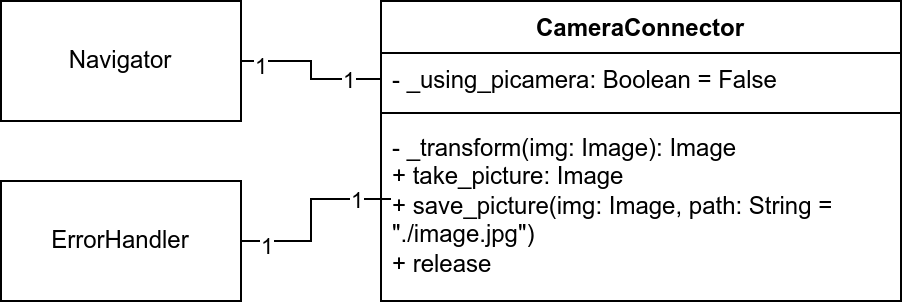
\includegraphics[width= \textwidth ]{assets/IT/robot-sw-architecture-camera-connector.png}
\caption{Kamera Modul}
\label{fig:camera-connector-classdiagram}
\end{figure}



\subsubsection{Ultraschall}
\label{ultraschall}

Zur Erhöhung der Betriebssicherheit ist das Fahrzeug mit einer redundanten Hinderniserkennung zusätzlich zu der Kamera ausgestattet. Diese erfolgt über einen Ultraschallsensor, der kontinuierlich die Entfernung zu Objekten im unmittelbaren Umfeld misst. Der Sensor ist direkt mit dem Mikrocontroller \gls{tinyk22} verbunden.

Die Messwerte werden in Echtzeit ausgewertet. Sobald ein Objekt in einer Distanz von weniger als 15cm erkannt wird, hält der Roboter an, um Kollisionen zu vermeiden. Diese Distanz wurde gewählt, damit die Balance eingehalten wird zwischen 'zu viel' oder 'zu spät' erkennen. Es sollen nicht fälschlicherweise Objekte erkannt werden, jedoch sollen sie auch nicht zu spät erkannt werden. Die 15cm wurden gewählt, damit es sicher genug Zeit gibt, um die Motoren auszuschalten, da der Roboter schneller fährt, wenn kein Objekt erwartet wird. Dies ist aber auch deswegen so, da die Kamera benutzt wird, um das unerwartete Objekt zu deuten. Die Kamera braucht eine bestimmte Distanz, um eine mögliche Pylone zu erkennen, da diese möglichst ganz auf dem Bild sein sollte. Die Kamera kann Objekte bis zu 10cm vor dem Roboter erkennen. 


Wird ein unerwartetes Objekt erkennt, wird ein definierter Fehlercode generiert und über die serielle Schnittstelle an den Raspberry Pi übertragen. Der Raspberry Pi leitete entsprechende Massnahmen ein. Dies ist beschrieben in Tabelle \ref{table:statuscodes}.

Dies hilft dabei Risiko 12 (Objekte werden nicht erkannt), siehe Tabelle \ref{table:risks}, zu mitigieren, falls es passiert.



\subsubsection{YOLOv11-Model trainieren}

Damit der Roboter Pylonen, Knoten und Hindernissen erkennen kann, wird ein \gls{yolo} Model trainiert.
Es werden mehrere Models trainiert, die laufend miteinander verglichen werden. Der Prozess wie das finale Model gewählt wurde, ist im Anhang in Kapitel ``\nameref{model-evaluation}'' zu finden.

Das Model, das verwendet wird, deutet die Bilder in ihrer Originalgrösse und hat über alle Klassen (Pylonen, Knoten, Hindernisse) gute Ergebnisse.

Die folgenden Abbildungen zeigen einige Bilder, die das Model annotiert hat. Darauf ist zu sehen, wie genau es die einzelnen Objekte erkennen kann.

\begin{figure}[H]
  \centering
   \begin{minipage}[b]{0.28\textwidth}
    \centering
    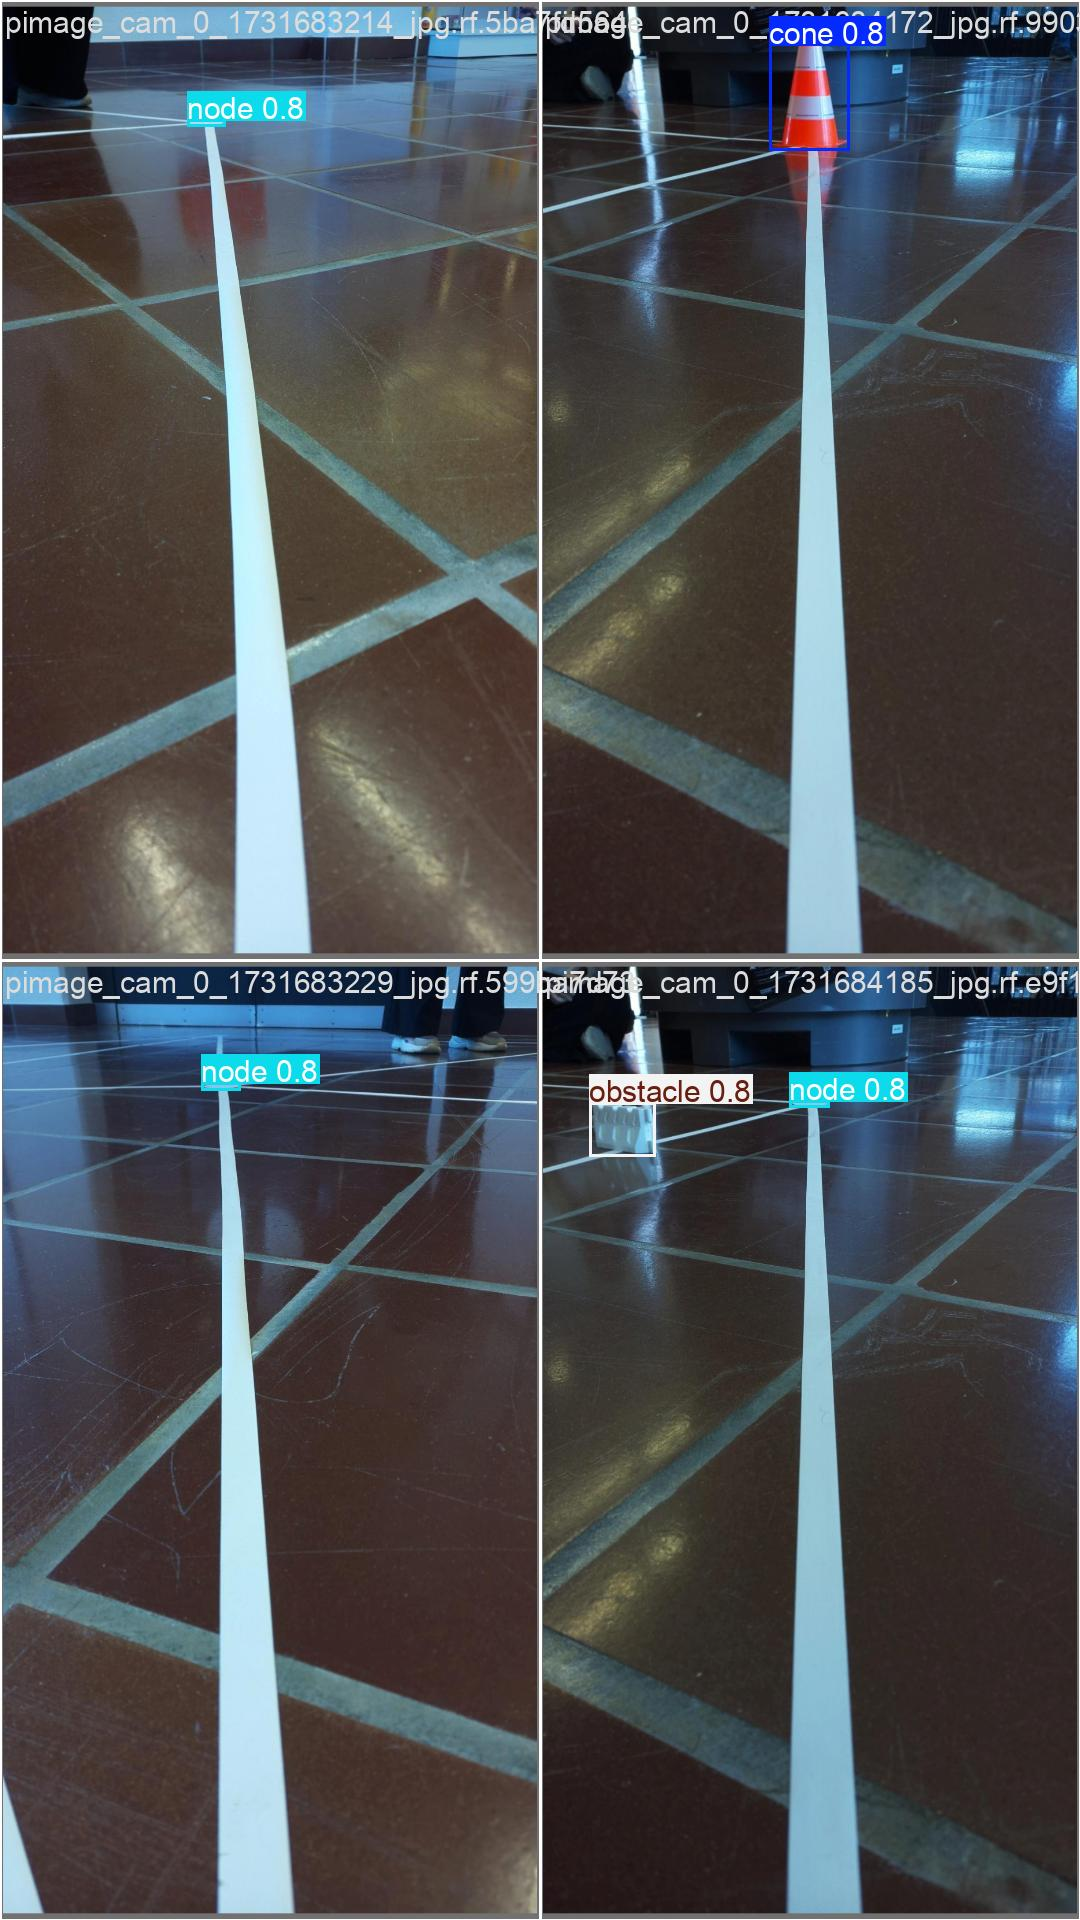
\includegraphics[width=\textwidth]{assets/IT/yolo/val_batch0_pred.jpg}
    \caption{Bilderkennung I}
    \label{fig:yolo-i}
  \end{minipage}
  \hfill
  \begin{minipage}[b]{0.28\textwidth}
    \centering
    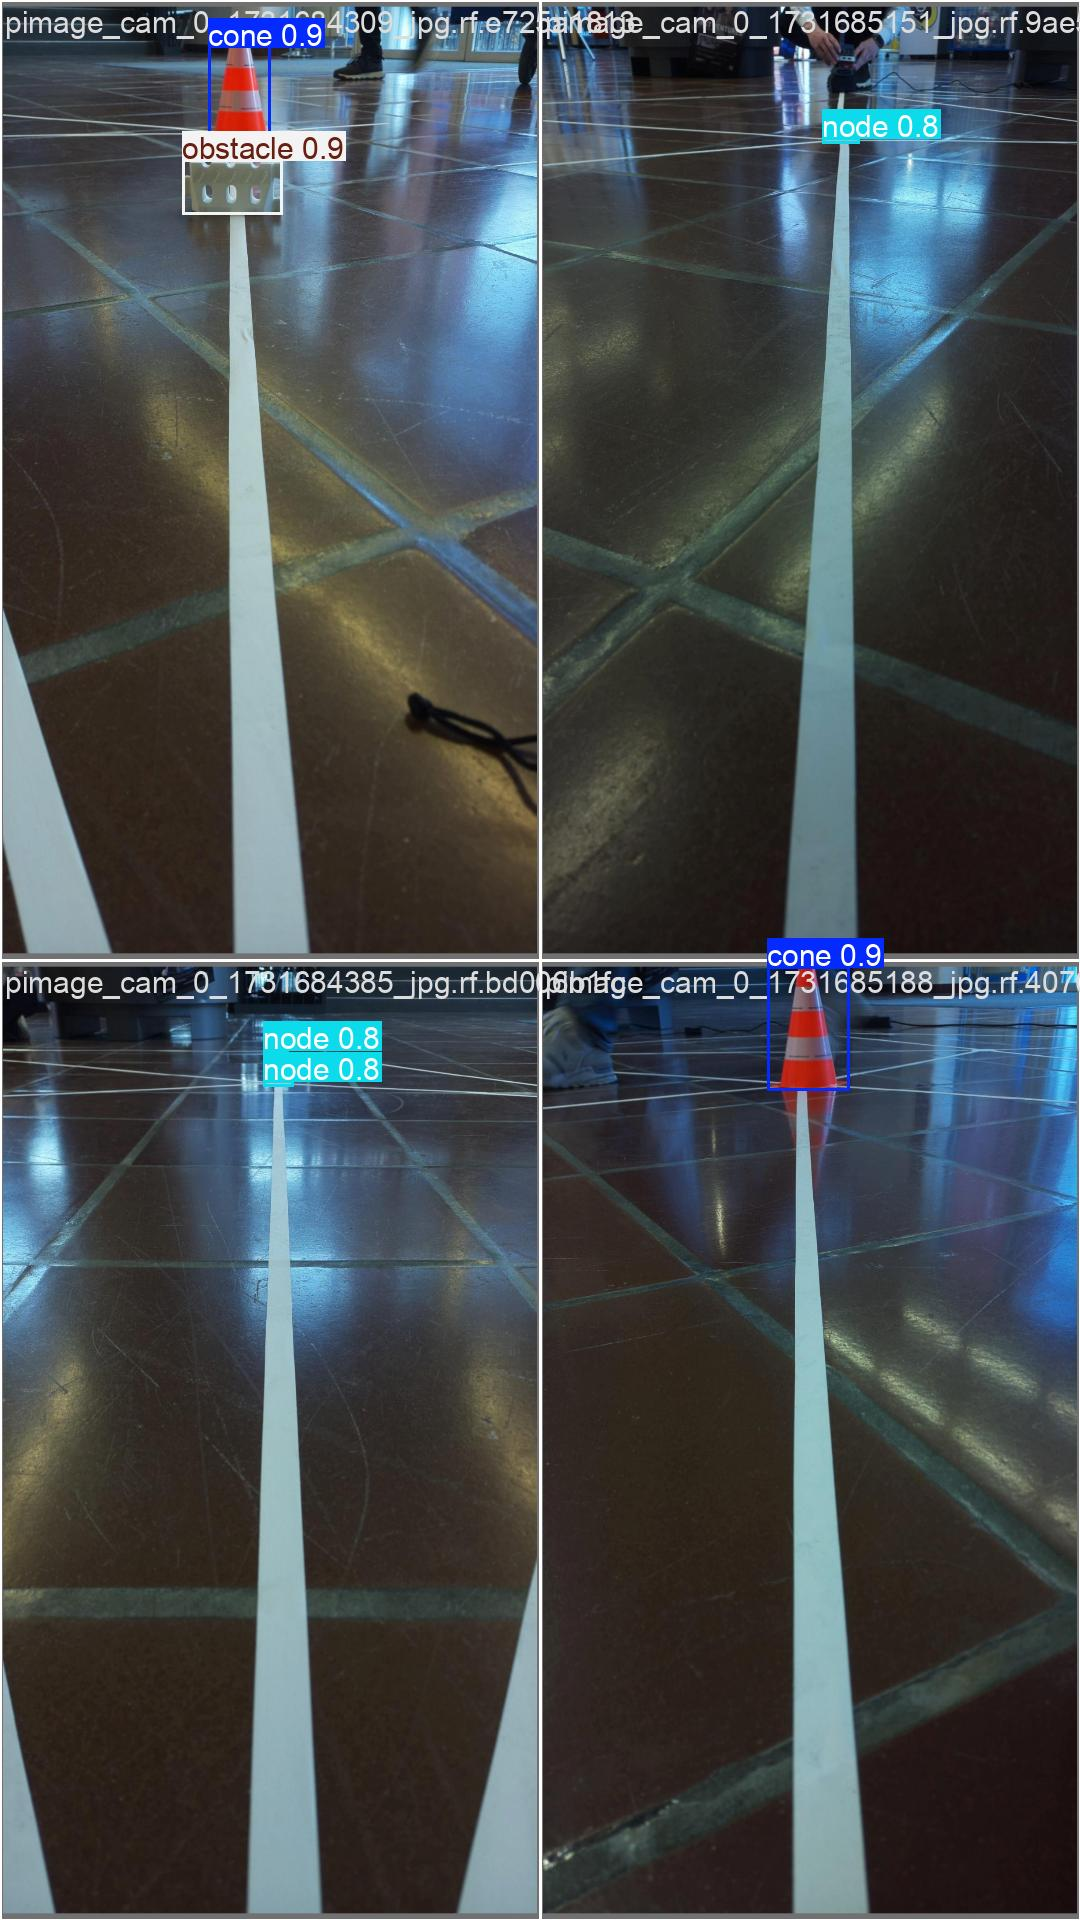
\includegraphics[width=\textwidth]{assets/IT/yolo/val_batch1_pred.jpg}
    \caption{Bilderkennung II}
    \label{fig:yolo-ii}
  \end{minipage}
    \hfill
  \begin{minipage}[b]{0.28\textwidth}
    \centering
    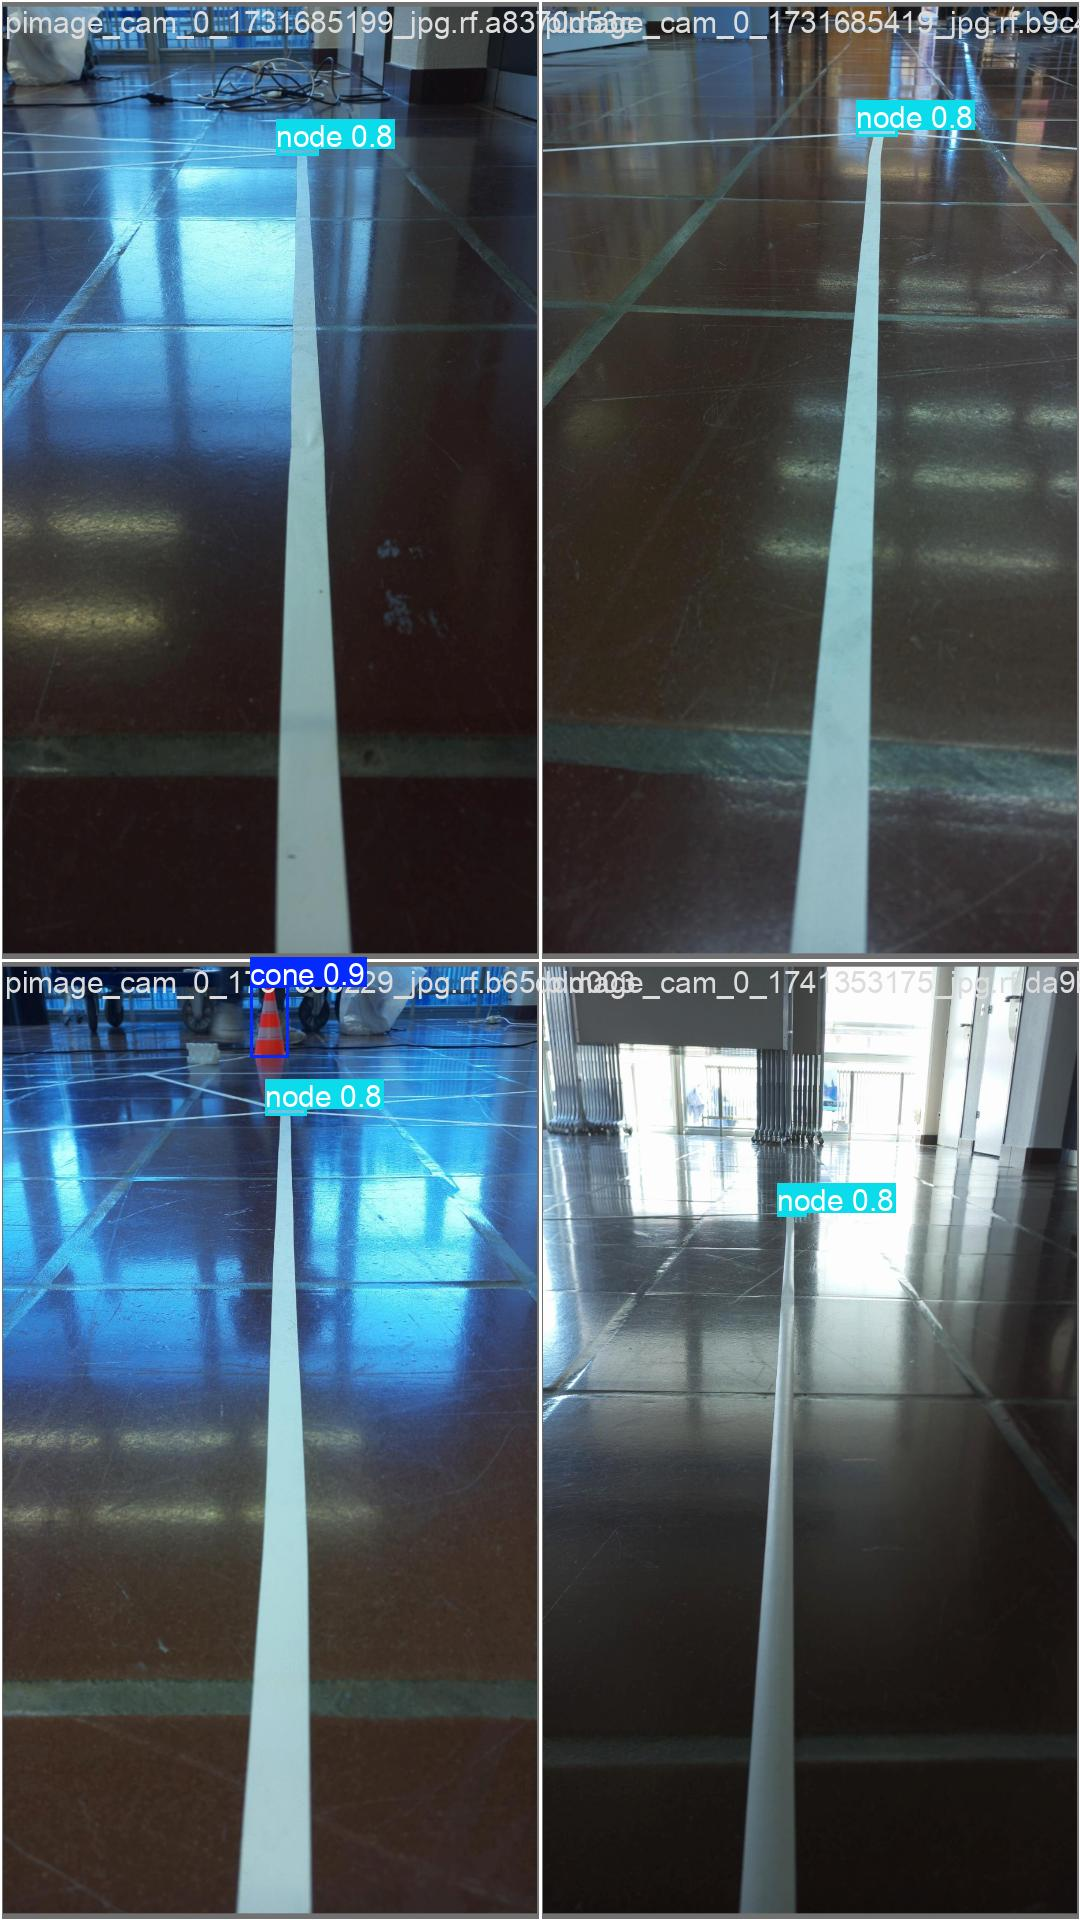
\includegraphics[width=\textwidth]{assets/IT/yolo/val_batch2_pred.jpg}
    \caption{Bilderkennung III}
    \label{fig:yolo-iii}
  \end{minipage}
\end{figure}

Auf den folgenden Bildern sind die Metriken aufgezeigt. Diese sind ebenfalls im Anhang im Kapitel ``\nameref{model-evaluation}'' genauer erklärt. 

Die Confusion Matrix ist auf Abbildung \ref{fig:conf-matrix}, diese zeigt, welche Objekte das Model wie oft falsch oder richtig gedeutet hat. Das Model hat jede Pylone und jede Barriere erkannt, hat sich zwei Knoten eingebildet und zwei Knoten verpasst. Mit den Algorithmen, die in dem nachfolgenden Kapitel \ref{model-results} beschrieben sind, die die Modelperformance stützen, sind diese Resultate ausgezeichnet. 


\begin{figure}[H]
    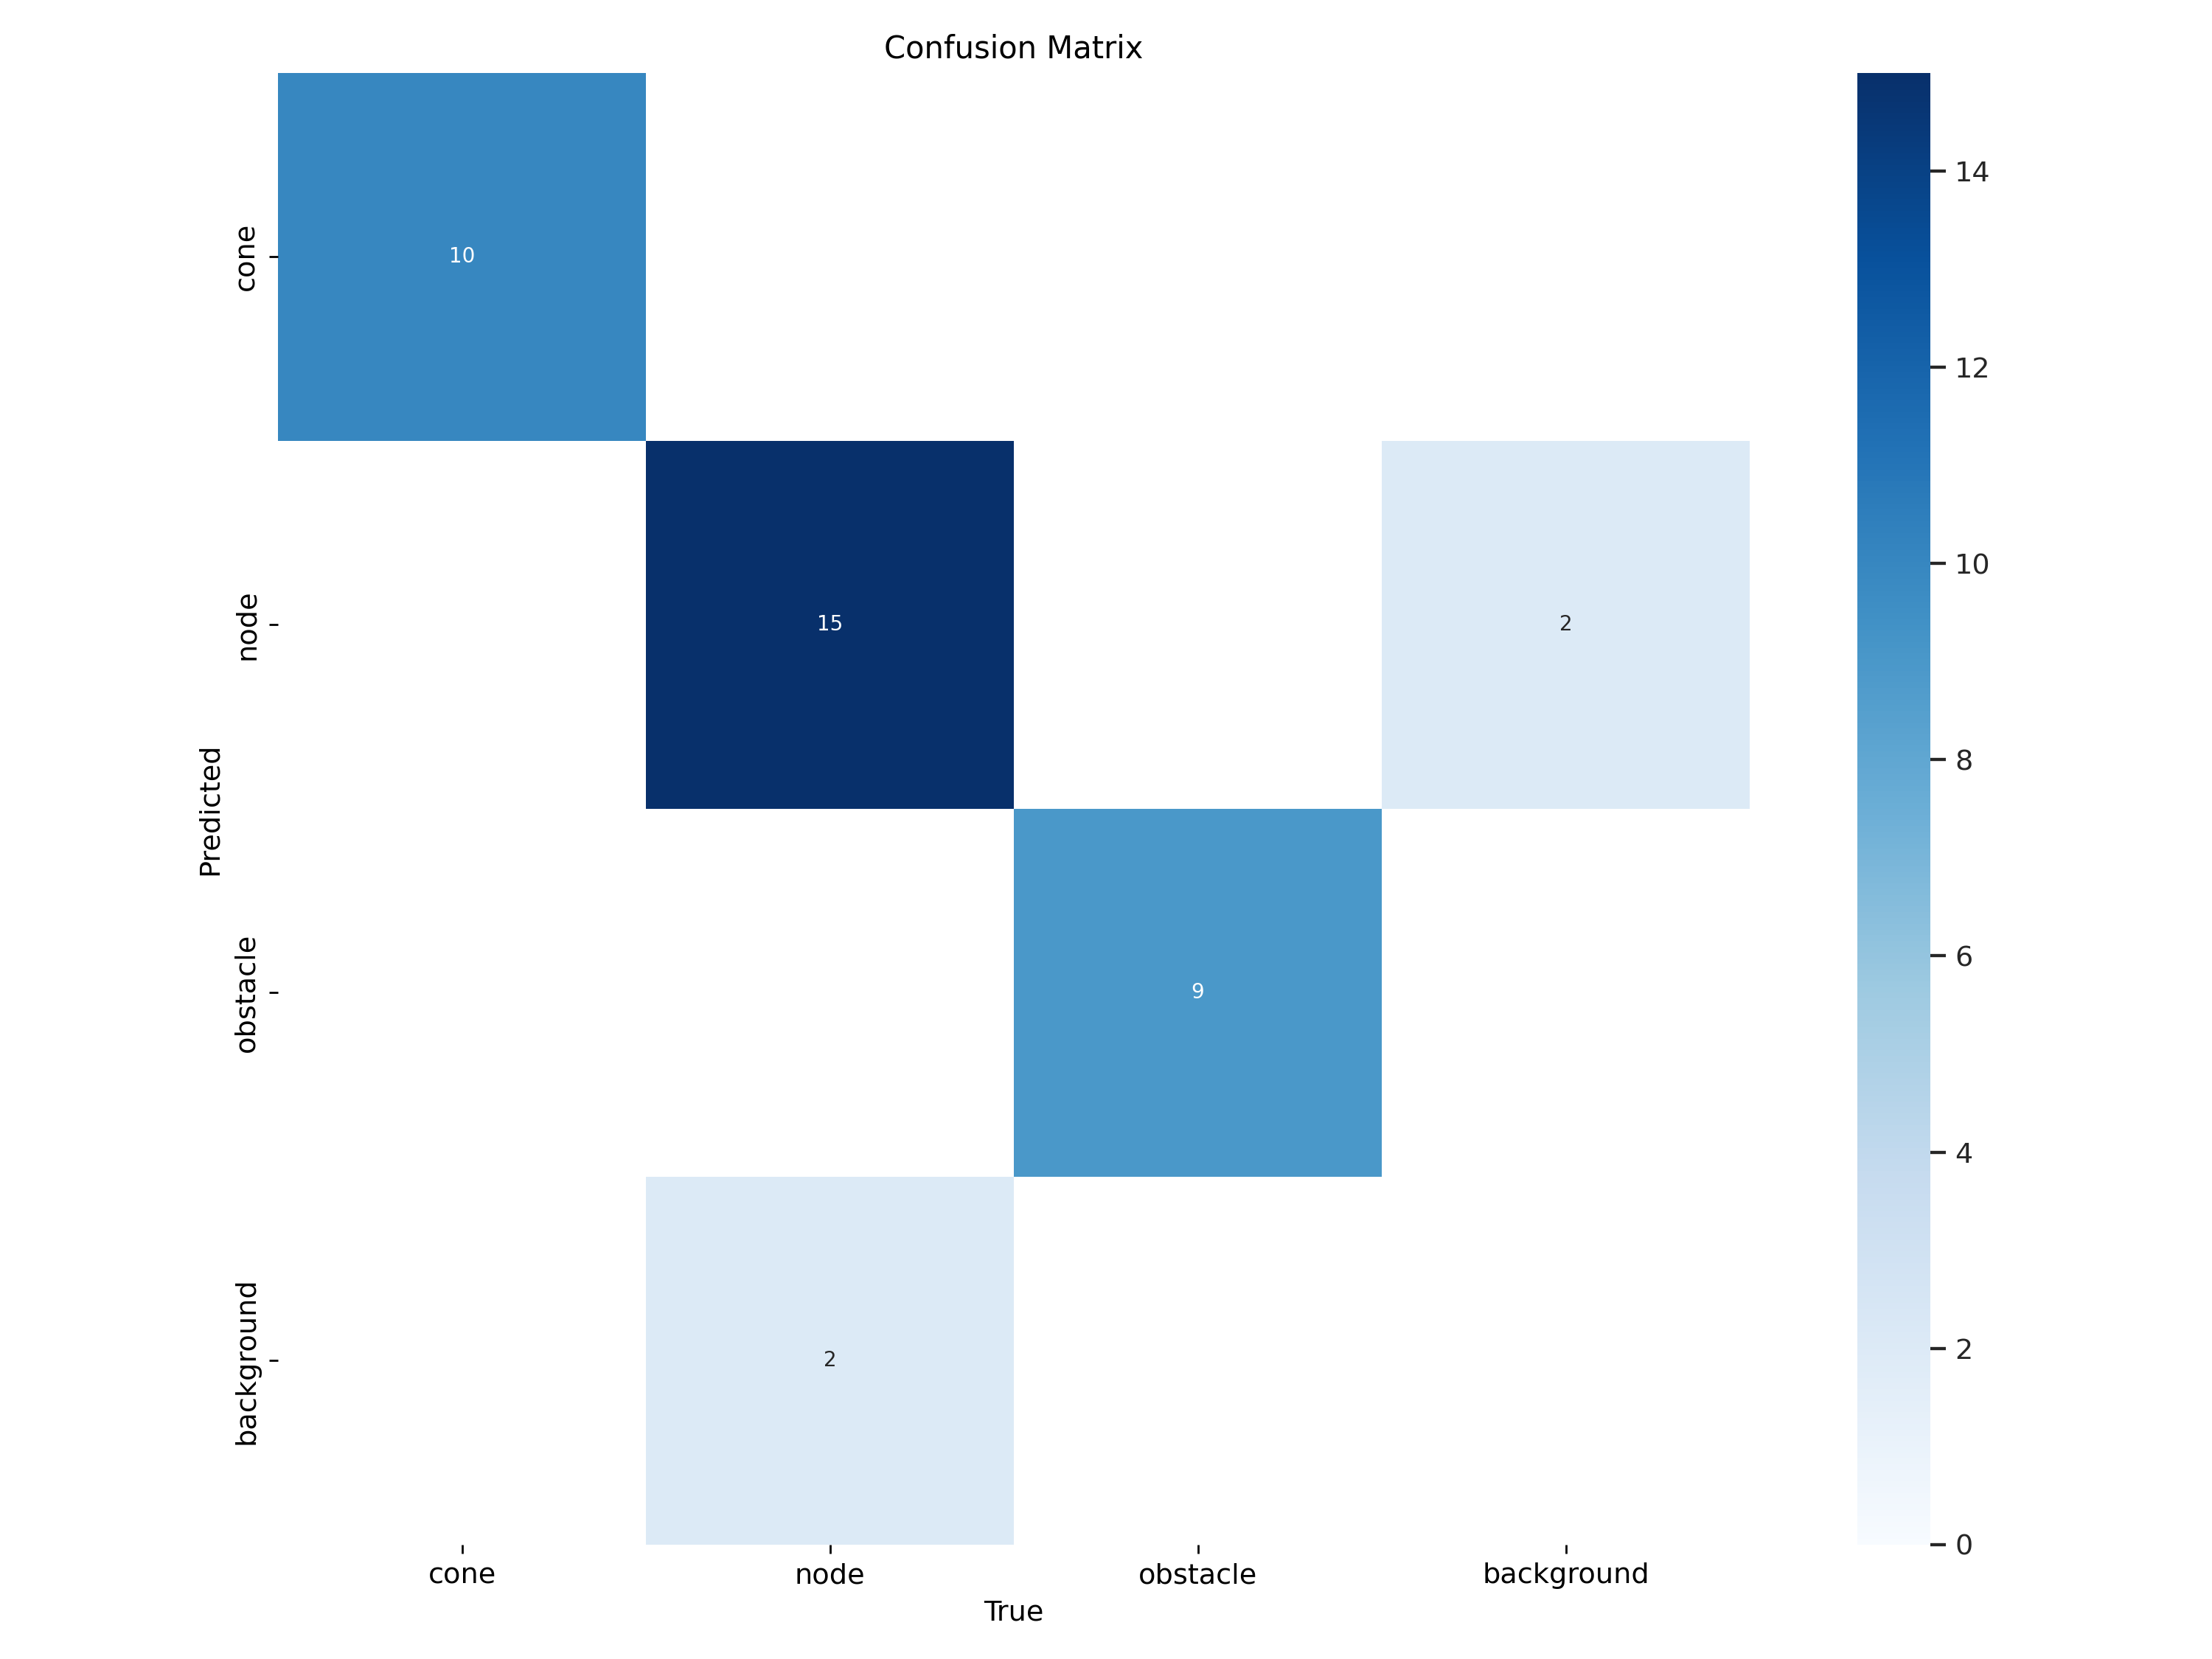
\includegraphics[width=\textwidth]{assets/IT/yolo/confusion_matrix.png}
    \caption{Confusion Matrix}
    \label{fig:conf-matrix}
\end{figure}

Was in Abbildung \ref{fig:f1}  sichtbar ist, ist der F1 Wert. Dieser ist besser, je höher er ist. Er ist hier für alle Klassen sehr hoch, was auf eine hohe Genauigkeit in den Detektierungen deutet. In Abblidung \ref{fig:results-lernverlauf} ist der Lernverlauf des Models ersichtlich. Alle Graphen zeigen das gewünschte Muster. Die 6 Graphen links, die den Verlust von falschen Deutungen darstellen, sind exponentiell fallend. Das heisst, dass das Modell mit jeder Iteration mehr gelernt hat und nicht irgendwann gestoppt hat oder schlechter wurde. Die 4 Graphen auf der rechten Seite zeigen, wie viel das Model gelernt, diese steigen und flachen dann ab. Dies ist ebenfalls das Muster, das bei einem guten Model erwartet wird.\cite{model-performance}


\begin{figure}[H]
    \begin{minipage}[b]{0.48\textwidth}
    \centering
    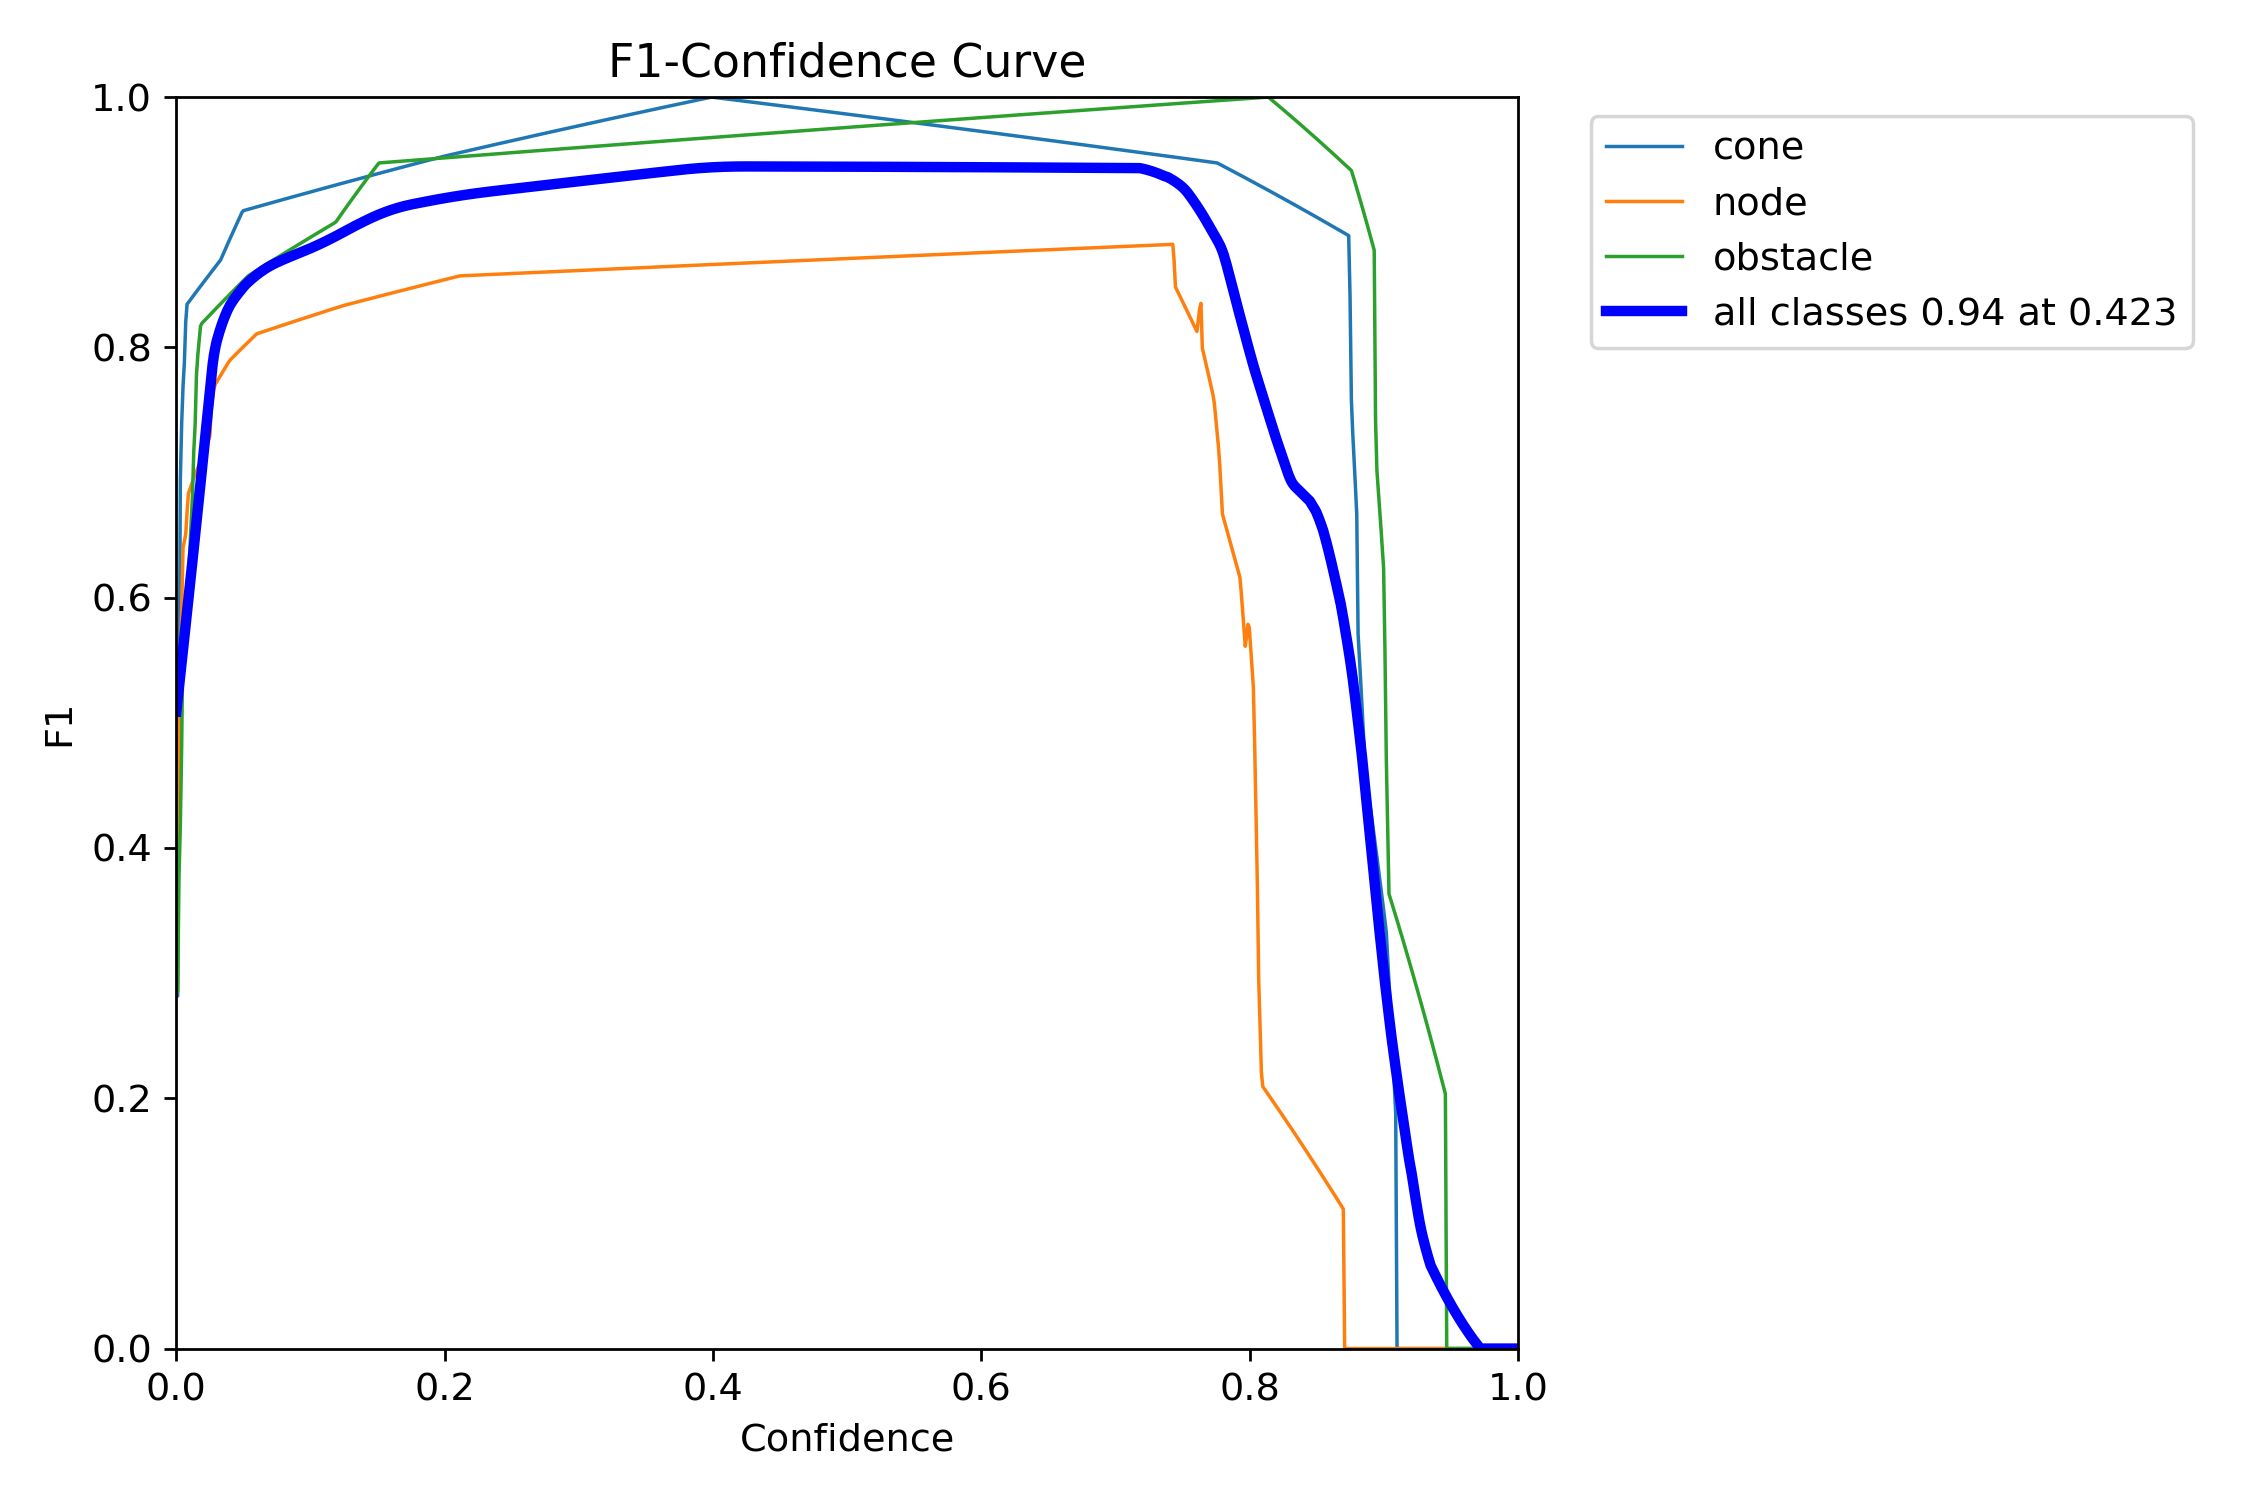
\includegraphics[width=\textwidth]{assets/IT/yolo/F1_curve.png}
    \caption{F1 Kurve}
    \label{fig:f1}
  \end{minipage}
    \hfill
  \begin{minipage}[b]{0.48\textwidth}
    \centering
    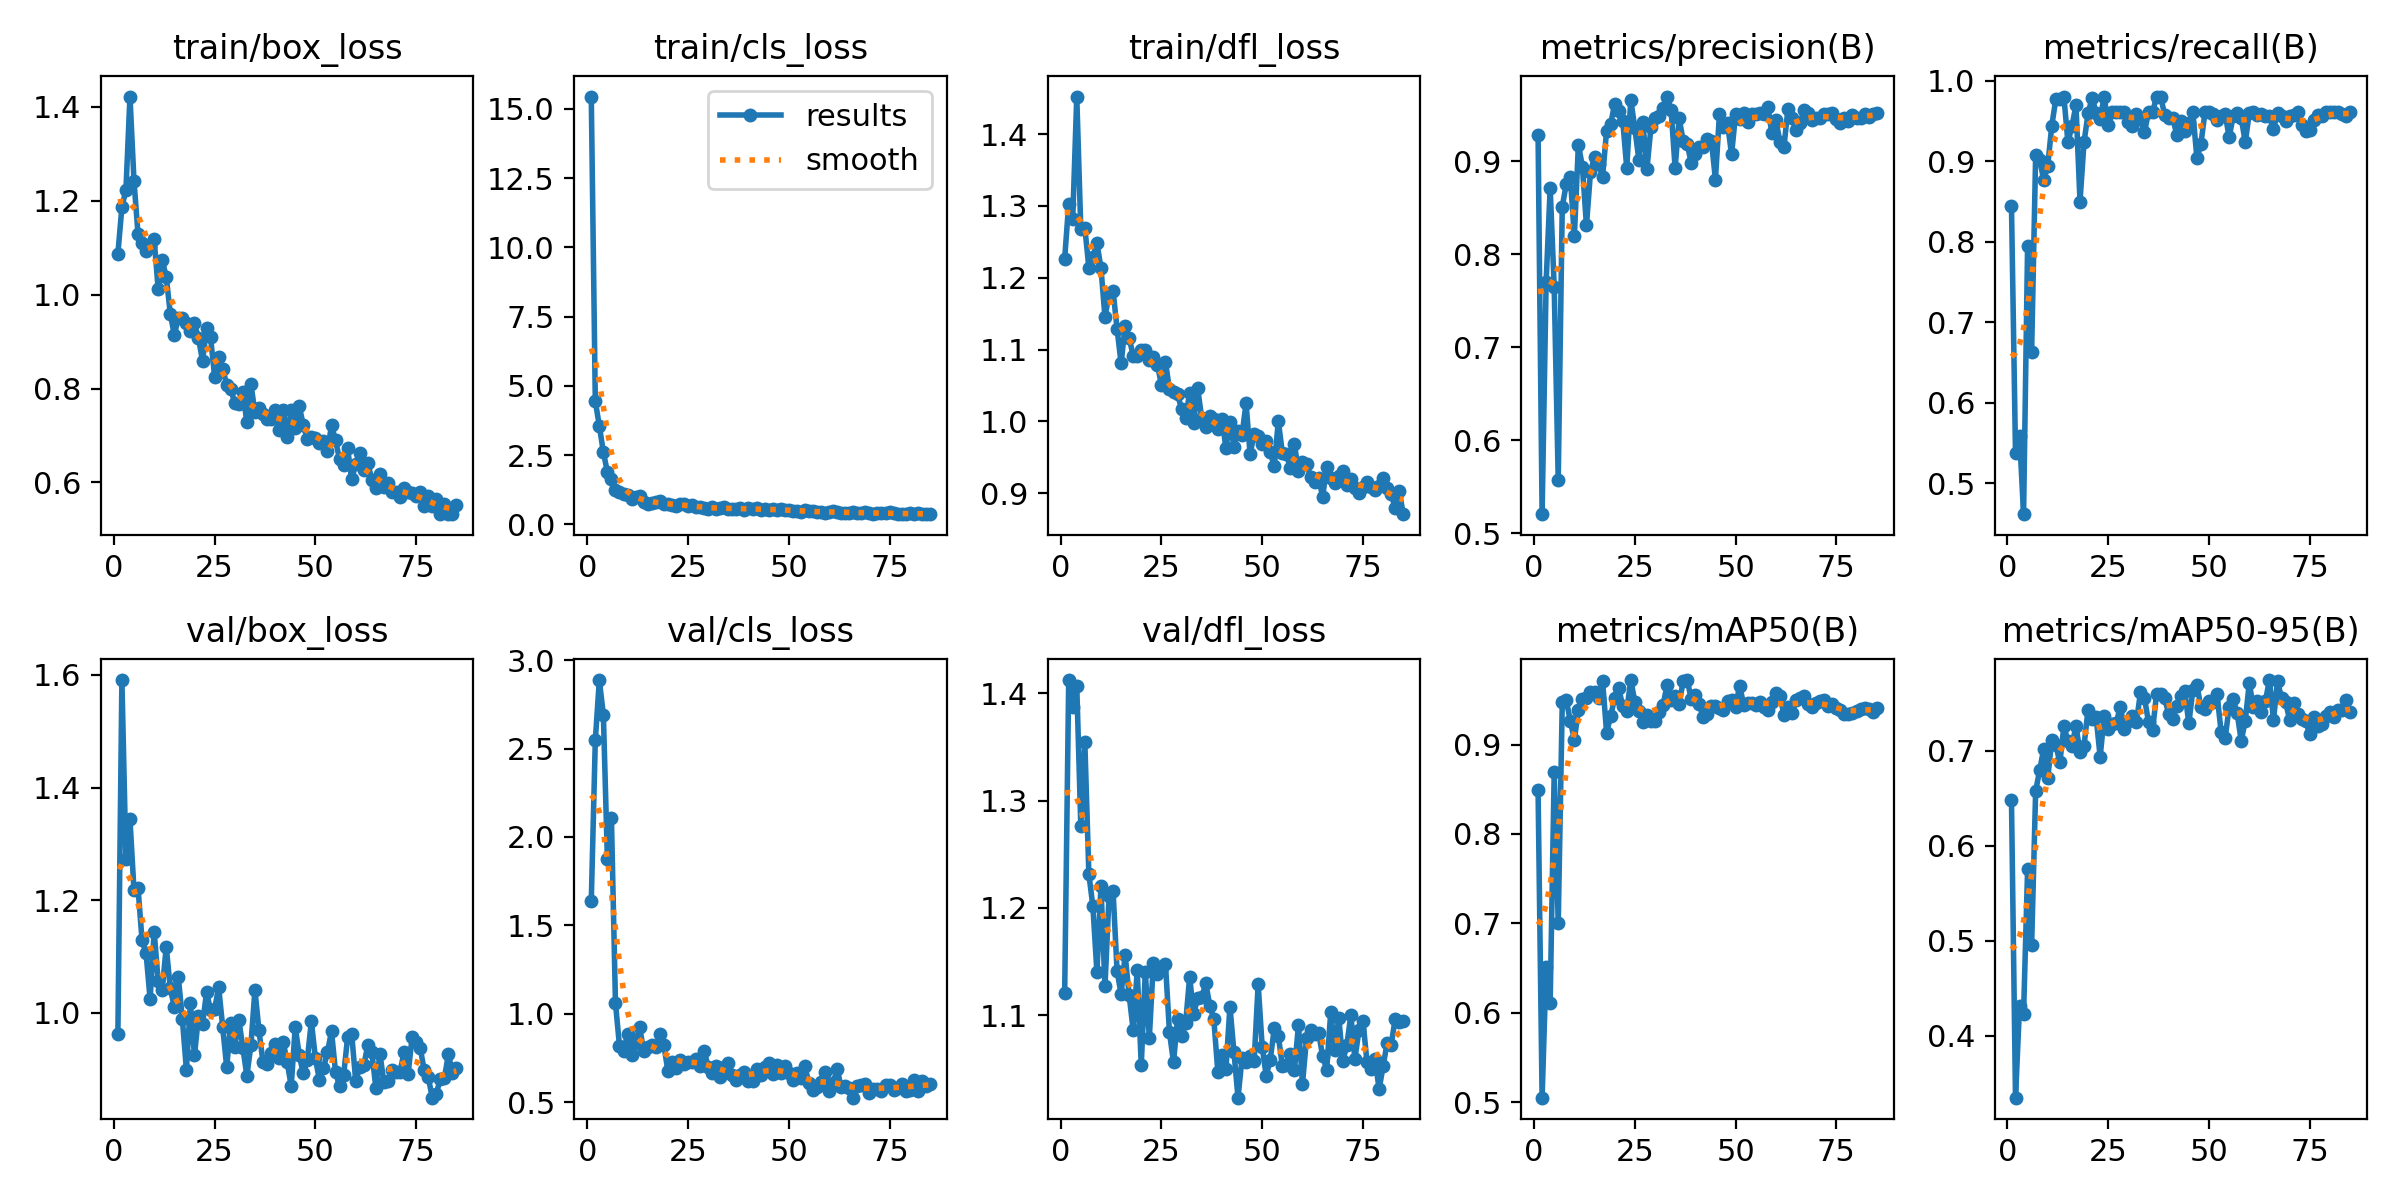
\includegraphics[width=\textwidth]{assets/IT/yolo/results.png}
    \caption{Lernverlauf}
    \label{fig:results-lernverlauf}
  \end{minipage}
\end{figure}

\subsubsection{YOLOv11 Model konvertieren}
\label{convert-yolo}

Es gibt Methoden, um die .pt Datei, das Format in welchem das Model gespeichert wird, mit der Ultralytics Bibliothek in ein anderes Format zu transformieren. Dadurch kann auf Embedded Systems und somit auch auf Raspberry Pi's die Bilderkennung schneller durchgeführt werden.

Drei Möglichkeiten wurden betrachtet und verglichen:

\begin{enumerate}
    \item Caffe2\footnote{\url{https://caffe2.ai/}}: In der Vergangenheit sehr geeignet, heutzutage mit PyTorch zusammengefügt und existiert nicht mehr auf diese Weise.\cite{caffe2}
    \item \acrfull{ncnn}\footnote{\url{https://docs.ultralytics.com/integrations/ncnn/}}: Sehr gute Performance für ARM Geräte (u.a. Raspberry Pi), sehr wenig Abhängigkeiten, einfache Transformation.\cite{ncnn-bib}
    \item \acrfull{onnx}\footnote{\url{https://onnx.ai/}}: Geeignet für  Cross-Plattform Fälle, gute Austauschbarkeit des Models, flexibel, viele Abhängigkeiten.\cite{onnx-bib}
\end{enumerate}

Es wird NCNN gewählt, da dies perfekt für den Verwendungszweck mit einem Raspberry Pi passt. Das erstellte .pt File kann mit der ultralytics Bibliothek transformiert werden:

\begin{verbatim}
yolo export model=best.pt format=ncnn
\end{verbatim}

Das Resultat ist ein Ordner, der gleich verwendet werden kann, wie das .pt File: Die Ultralytics Library erwartet den Pfad zu der Datei, respektive dem Ordner und baut daraus das YOLO Model, welches in Python verwendet werden kann. Mit der Transformation wurde das Risiko 3 (4 Minuten reichen nicht für einen Durchgang) (siehe Tabelle \ref{table:risks}), weiter gemindert. Auf dem Raspberry Pi, kann die Bilderkennung pro Bild konstant unter einer Sekunde gehalten werden.

\subsubsection{Modelresultate auswerten}
\label{model-results}

Um die Modelresultate auszuwerten, wird das Model in den Ordner der Navigation kopiert und es wird eine ObjectDetector Klasse und ein Object Enum erstellt, gezeigt im Klassendiagramm auf Abbildung \ref{fig:nav-object-detector}.

 \begin{figure}[H]
\centering
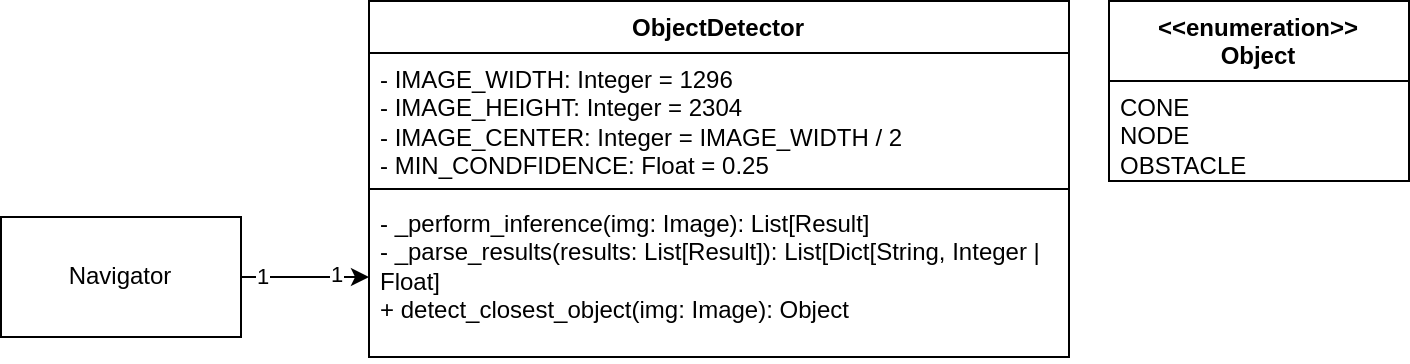
\includegraphics[width= \textwidth ]{assets/IT/robot-sw-architecture-object-detector.png}
\caption{Object Detector Modul}
\label{fig:nav-object-detector}
\end{figure}

Diese ObjectDetector Klasse ladet das Model bei der Instanzierung und wird aufgerufen, wenn ein Nachbarsknoten geprüft werden soll und führt einen Prozess von drei Schritten durch:

\begin{enumerate}
    \item Inference (Objekterkennung).
    \item Resultat parsen.
    \item Nächstes Objekt vor dem Roboter finden.
\end{enumerate}

Im Teil der Inference wird ein Bild an das Model gegeben. Dabei sollen nur diese erkannten Objekte zurückgegeben werden, die mit einer definierten prozentualen Gewissheit erkannt wurden. Diese Gewissheit ist als Konstante definiert auf 0.4. Aus der F1 Kurve in Abbildung \ref{fig:f1} kann gelesen werden, dass die Barriere bei 0.4 die besten Resultate hat. Knoten und Pylone sind recht konstant und haben dort ebenfalls sehr genaue Resultate. Dadurch, dass dieser Wert von dem Standardwert erhöht wurde, kann das Risiko 7 (Ein Objekt wird fälschlicherweise erkannt), siehe Tabelle \ref{table:risks}, damit vermindert werden: Das Modell muss sich sicherer sein, als dies standardmässig der Fall ist, damit die Deutung akzeptiert wird.

Diese Resultate werden dann geparsed, sodass alle erkannten Objekte mir ihrer ID, mit der Confidence, mit der sie erkannt wurden, und mit ihrem Standort auf dem Bild zurückgegeben werden.

Aus dieser Liste werden nun alle Objekte betrachtet, die sich auf der Mittellinie des Bildes befinden. Somit kann sichergestellt werden, dass nicht versehentlich Objekte, die sich nicht auf der Fahrbahn befinden, gespeichert werden und auch Risiko 7 (Objekte werden fälschlicherweise erkannt, siehe Tabelle \ref{table:risks}) kann so mitigiert werden. Die Mittellinie wird berechnet aus der Breite des Bildes. Die Objekte auf der Mittellinie werden sortiert nach ihren Koordinaten auf dem Bild. Das erste Element in dieser Liste ist das nächste Objekt zum Roboter.

In folgenden Fällen wird nicht einfach das nächste Objekt zurückgegeben:

\begin{itemize}
    \item Falls das nächste Objekt eine Barriere und das zweitnächste eine Pylone ist. In diesem Fall wird zurückgegeben, dass eine Pylone das nächste Objekt ist, da dieser Knoten sowieso nicht befahrbar ist und aus dem internen Graph entfernt werden soll.
    \item Falls kein Objekt erkannt wurde, wird ein Knoten zurückgegeben. Es ist weniger wahrscheinlich, dass eine Barriere oder ein Pylon verpasst werden, als dass ein Knoten nicht erkannt wird. Somit wird Risiko 2 (Knoten werden nicht erkannt, siehe Tabelle \ref{table:risks}) behandelt. Der Ultraschall kann trotzdem Objekte noch erkennen, falls ein Objekt verpasst wurde. Durch den Ultraschall werden Risiko 12 und 1 (Objekte werden nicht erkannt, siehe Tabelle \ref{table:risks}) mitigiert.
\end{itemize}

Die folgenden Abbildungen veranschaulichen das Prinzip. Diese Bilder haben die einzelnen Objekte, die das Model erkannt hat mit Boxen annotiert. Die Bildunterschrift zeigt, welche Objekte zurückgegeben werden, basierend auf dem Algorithmus, der zuvor erklärt wurde. Wenn es keine Box annotiert hätte, würde ebenfalls ein Knoten zurückgegeben werden.

\begin{figure}[H]
  \centering
    \begin{minipage}[b]{0.23\textwidth}
    \centering
    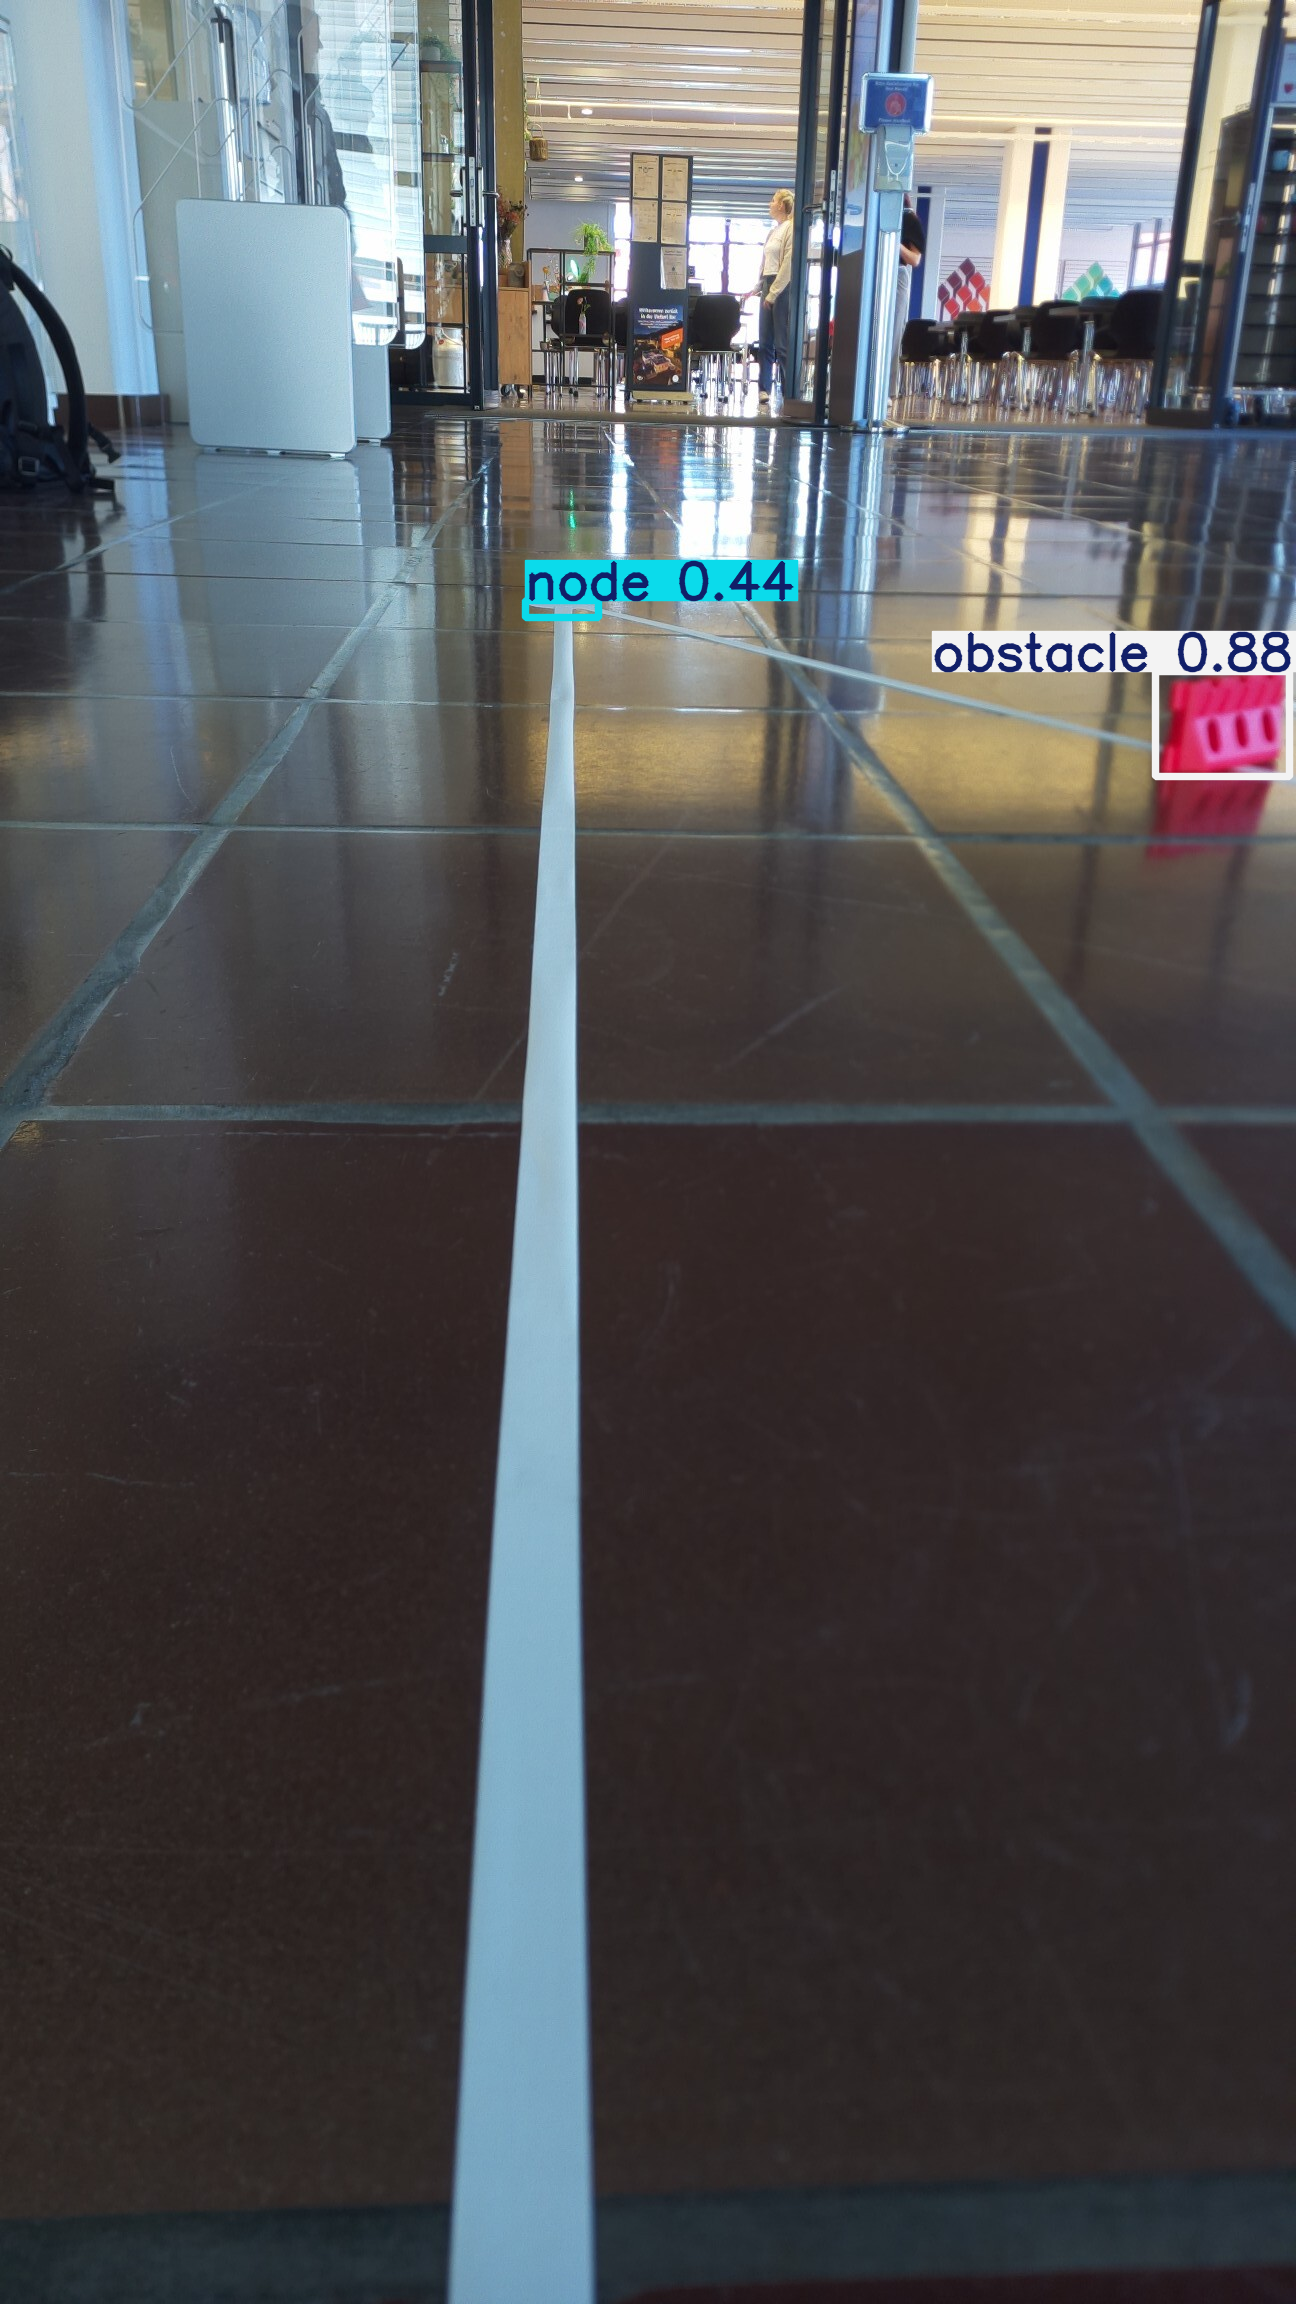
\includegraphics[width=\textwidth]{assets/IT/testing/yolo/node-obst-on-the-side_annot.png}
    \caption{Returned Knoten}
    \label{fig:expl-algo-1}
  \end{minipage}
  \hfill
  \begin{minipage}[b]{0.23\textwidth}
    \centering
    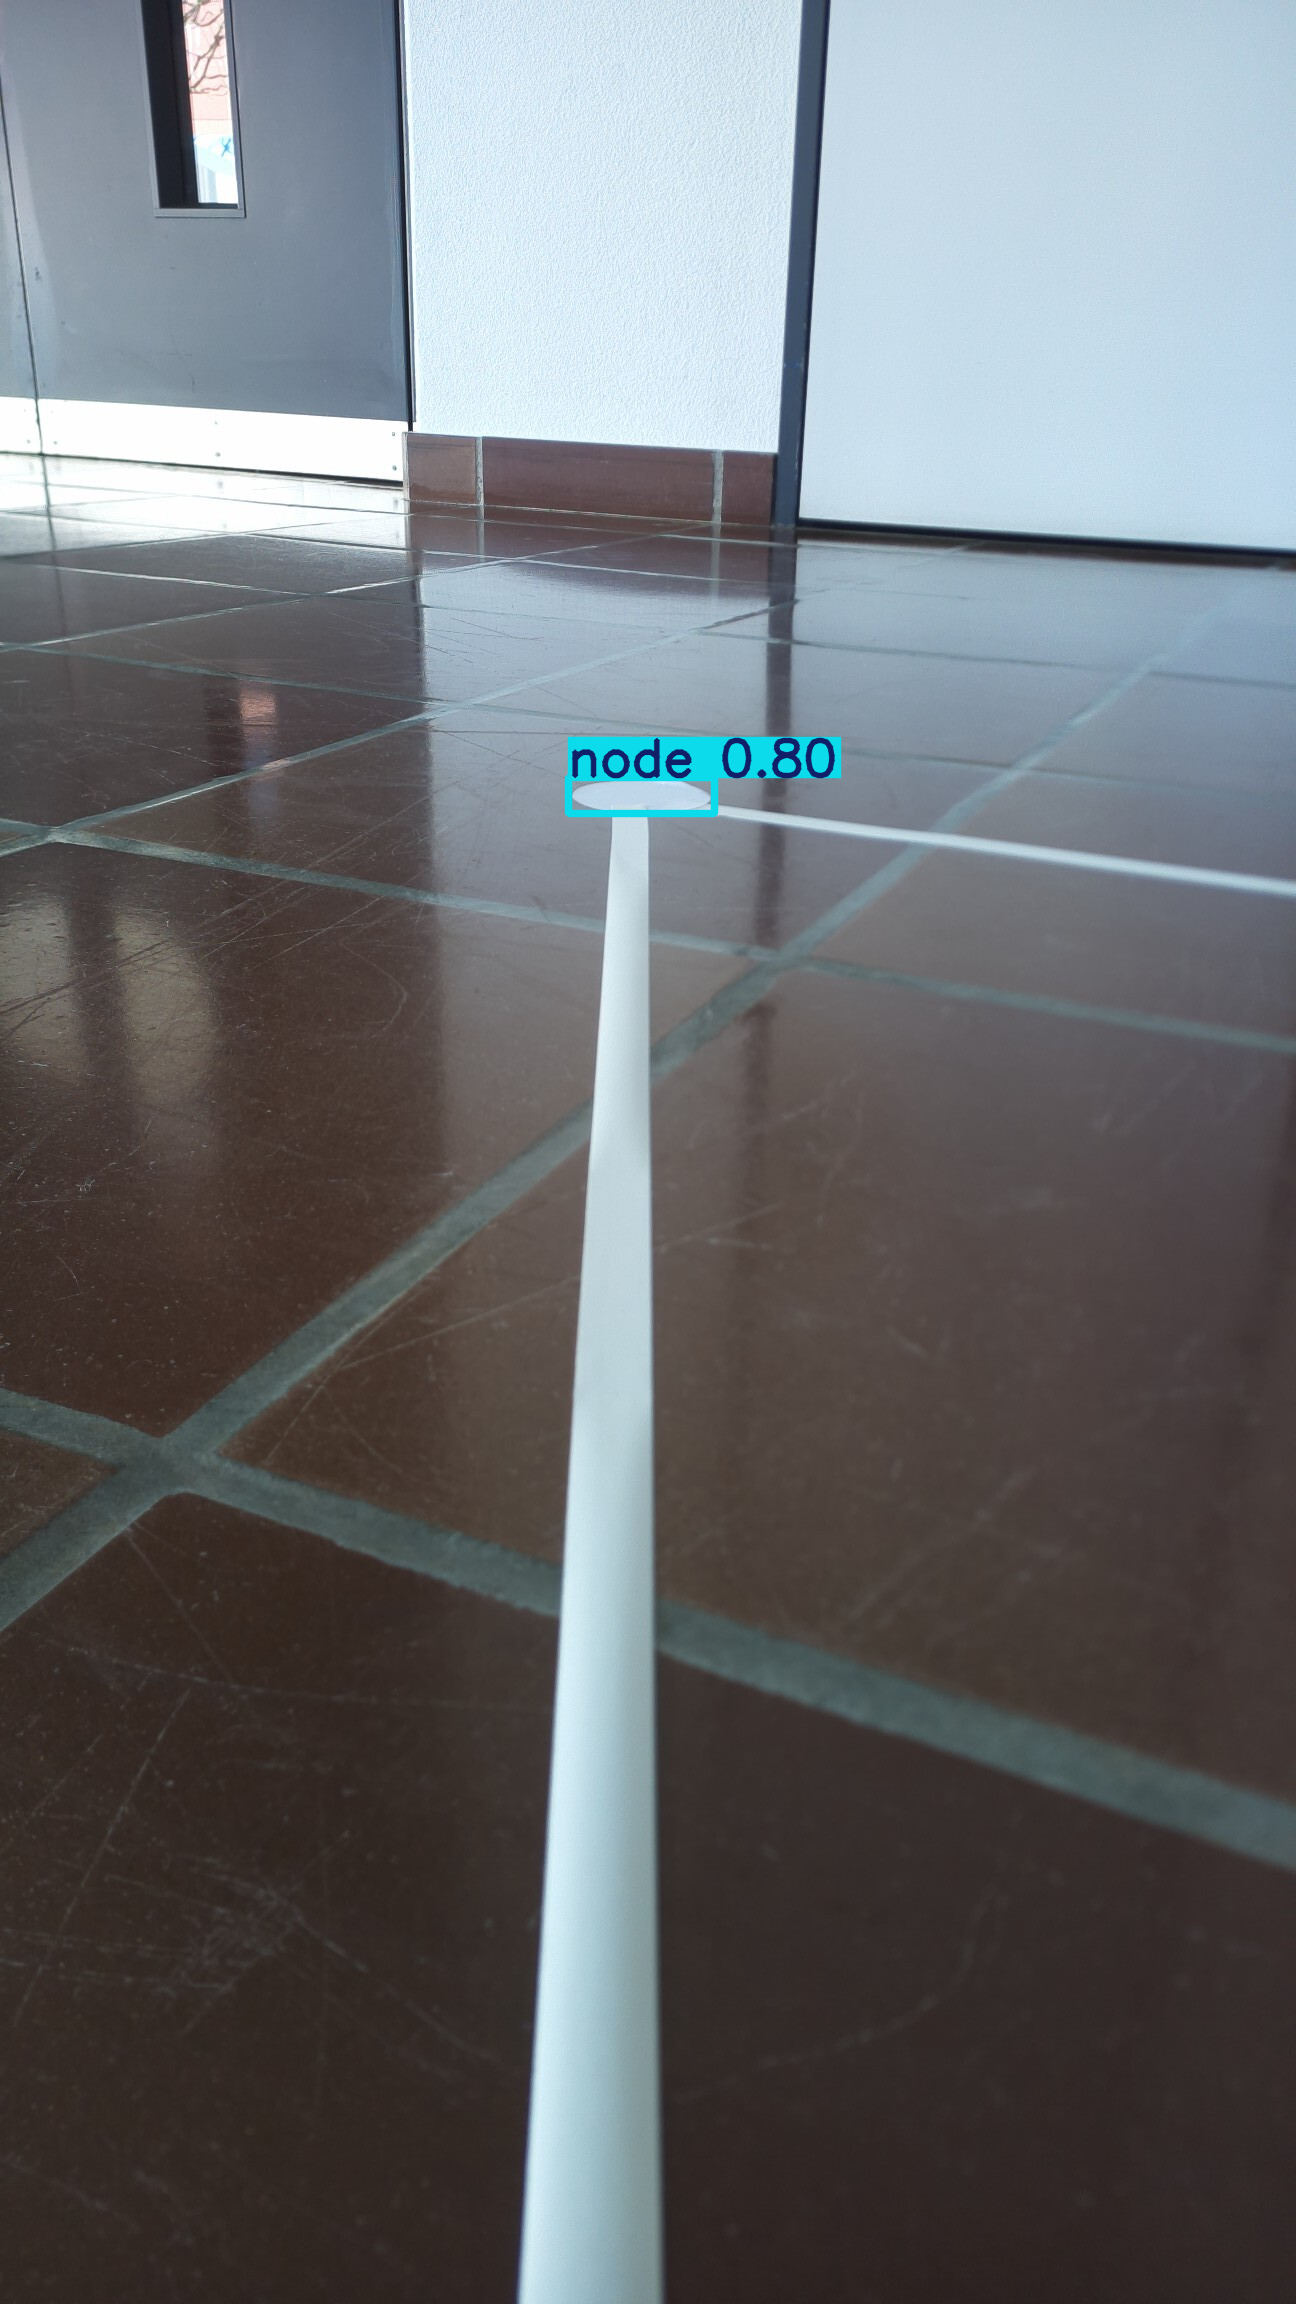
\includegraphics[width=\textwidth]{assets/IT/testing/yolo/node_annot.png}
    \caption{Returned Knoten}
    \label{fig:expl-algo-2}
  \end{minipage}
    \hfill
  \begin{minipage}[b]{0.23\textwidth}
    \centering
    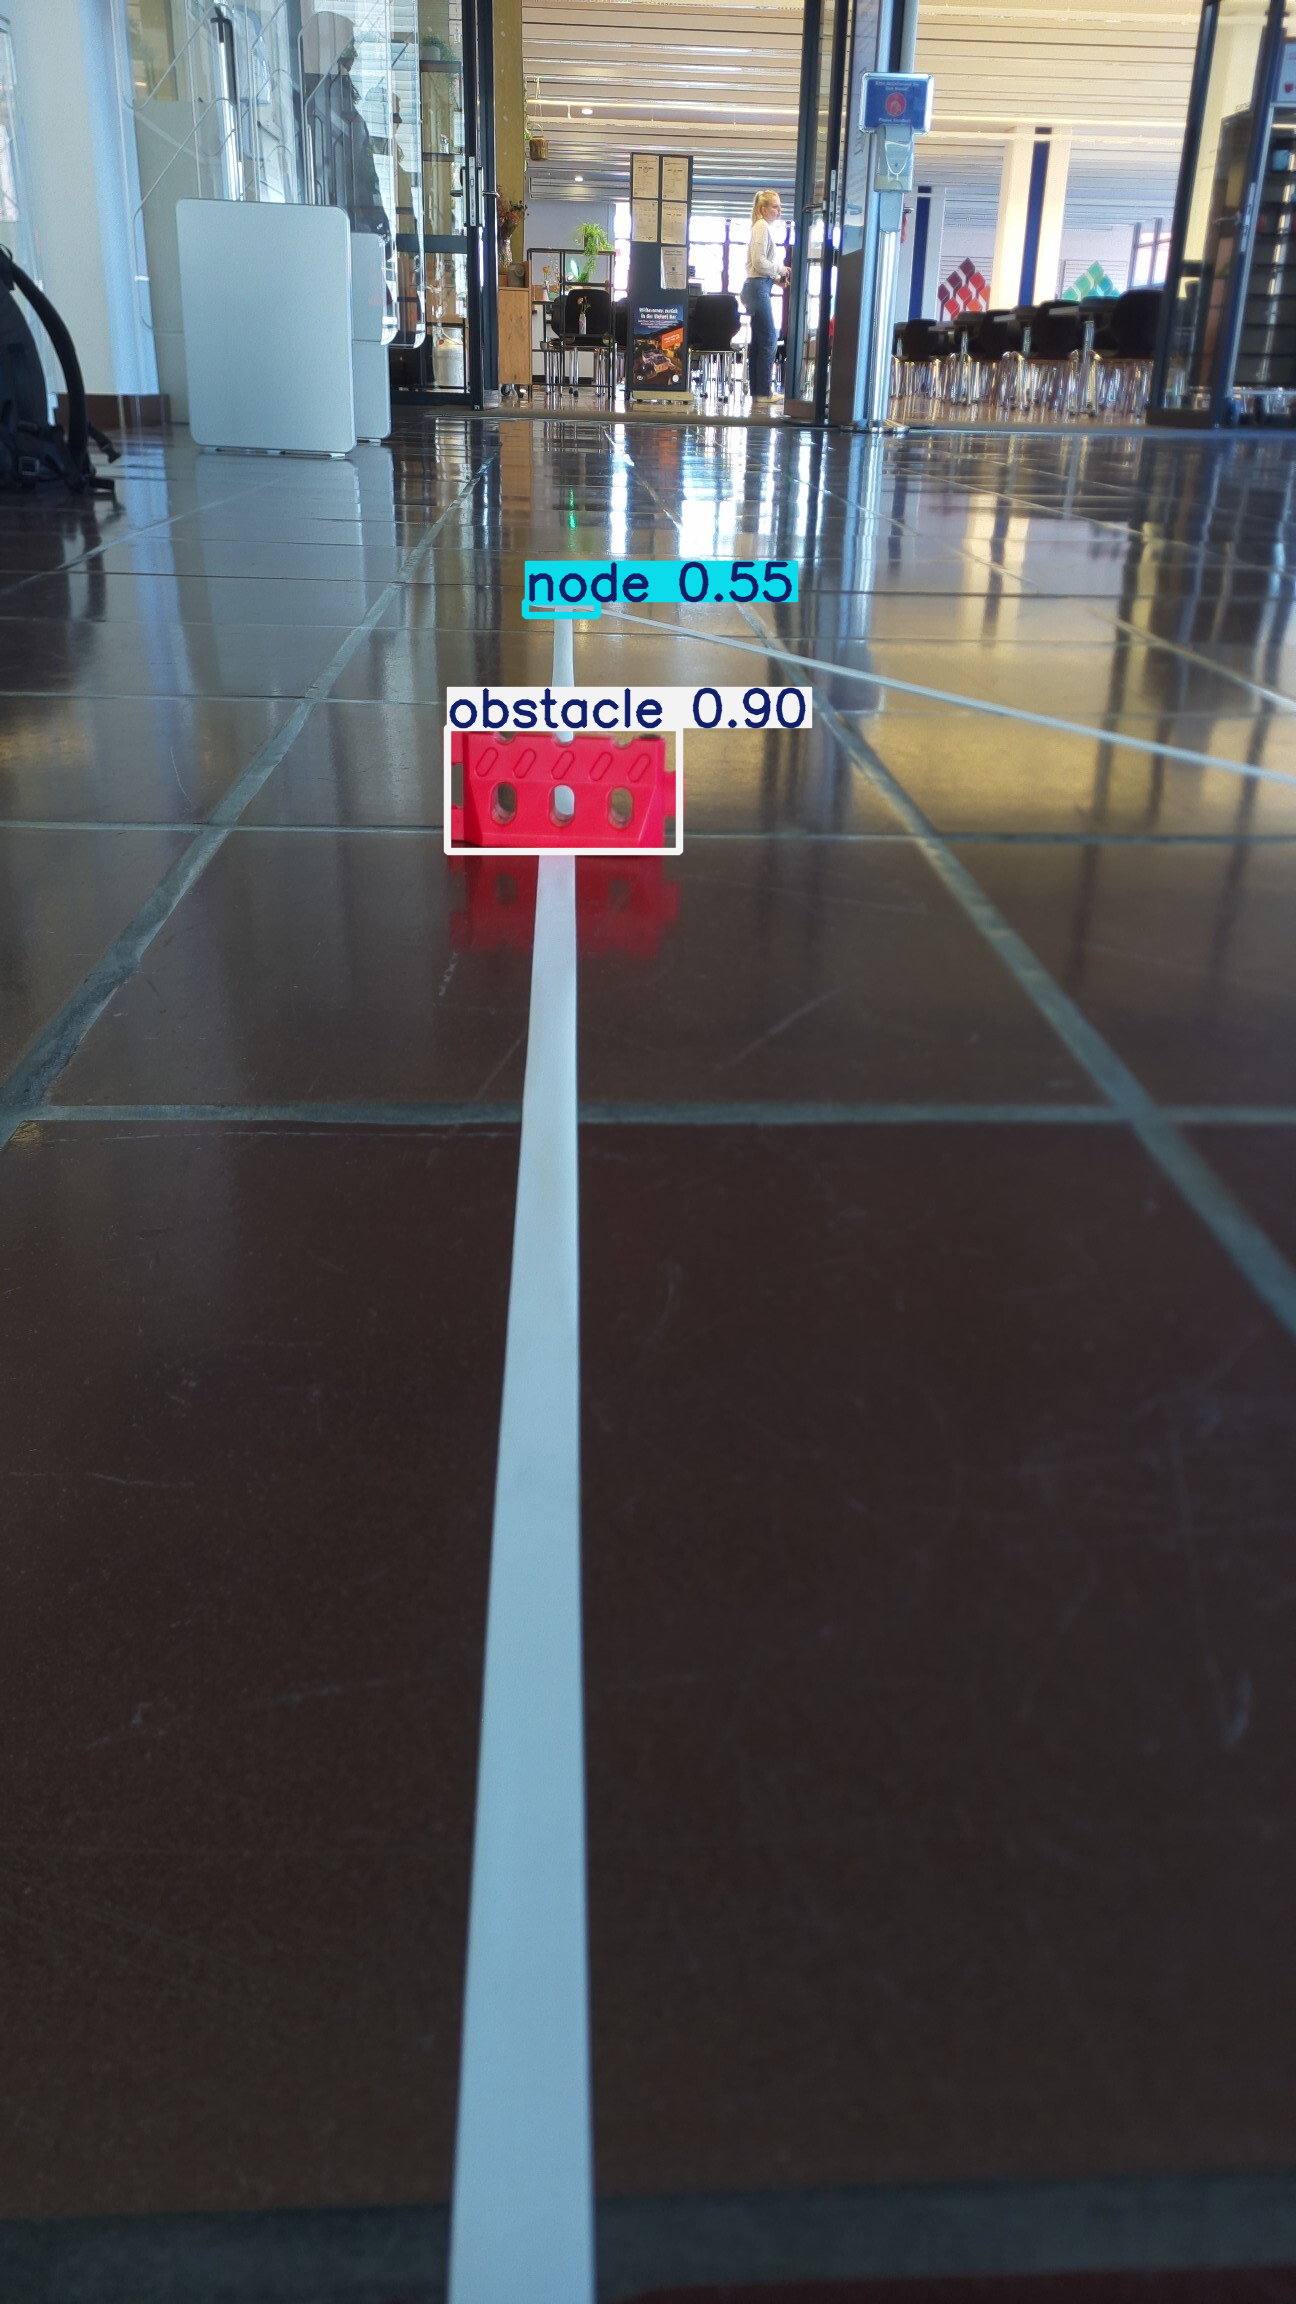
\includegraphics[width=\textwidth]{assets/IT/testing/yolo/barrier_annot.png}
    \caption{Returned Barriere}
    \label{fig:expl-algo-3}
  \end{minipage}
      \hfill
  \begin{minipage}[b]{0.23\textwidth}
    \centering
    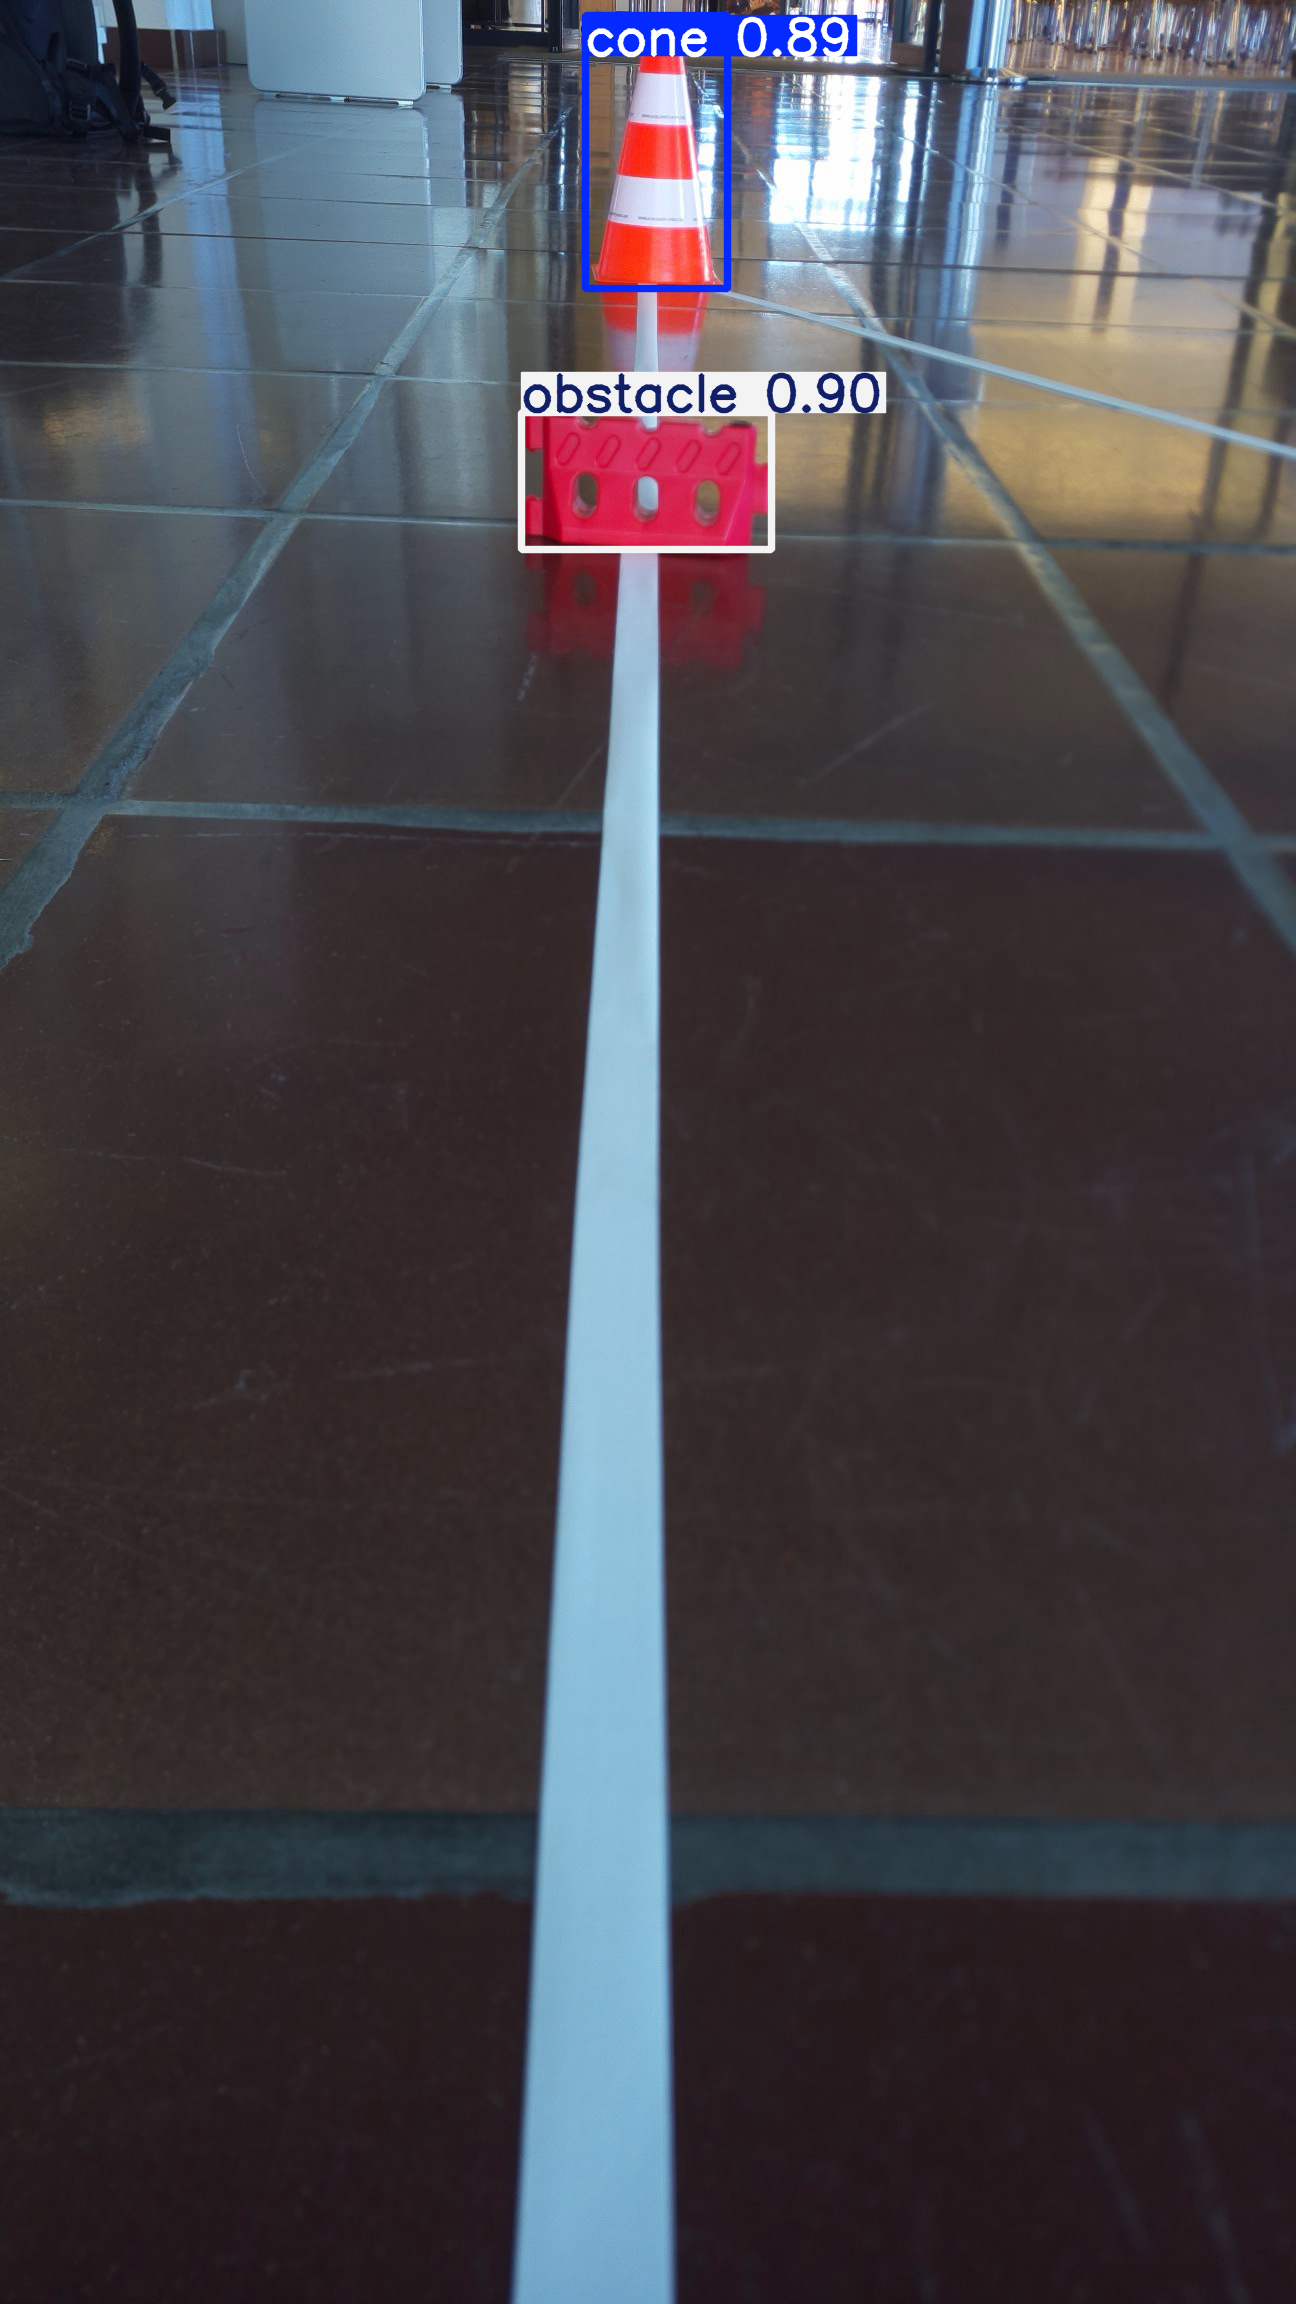
\includegraphics[width=\textwidth]{assets/IT/testing/yolo/pylon_behind_obst_annot.png}
    \caption{Returned Pylone}
    \label{fig:expl-algo-4}
  \end{minipage}
\end{figure}

Wie auf die einzelnen Objekte reagiert wird, ist in folgender Aufzählung beschrieben und ist gleich, wie in \acrshort{pren1} geplant.

\textbf{Pylonen erkennen}

Wird eine Pylone erkannt, wird der Knoten, der gerade geprüft wurde, inklusive alle Strecken dahin, aus dem internen Graphen entfernt.

\textbf{Knoten erkennen}

Wenn ein Knoten erkannt wird, dann geschieht nichts. Es wird interpretiert, dass sich kein Objekt auf diesem Weg befindet und die Strecke normal befahrbar ist.

\textbf{Barrieren erkennen}

Wird auf dem Bild eine Barriere erkannt, wird dies im internen Graphen gespeichert, indem die jeweilige Linie höher gewichtet wird, da es länger dauern wird diese zu überqueren.

\textbf{Entfernte Linien erkennen}

Die entfernten Linien werden erkannt, wenn die Winkel der ausgehenden Linien berechnet wird, Details dazu, gibt es in Kapitel \ref{outgoing-lines}. Die fehlende Linie wird aus dem internen Graphen entfernt.

\newpage
%%%%%%%%%%%%%%%%%Epic 11%%%%%%%%%%%%%%%%%%%%%%%%%%%%%%%%%%%%%%%%%%%%%%%%%%%%%%%
\subsection{Zieleingabe: Peripherie Ein- und Ausgabe}

In diesem Kapitel wird die Ein- und Ausgabe des Roboters thematisiert.
Dafür wird auf dem Raspberry Pi ein Prototypen-HAT montiert, welcher die benötigten GPIO-Pins entsprechend der Abbildung \ref{fig:raspiheader-schema} auf Taster, Display und Buzzer verbindet.

\begin{figure}[H]
    \centering
    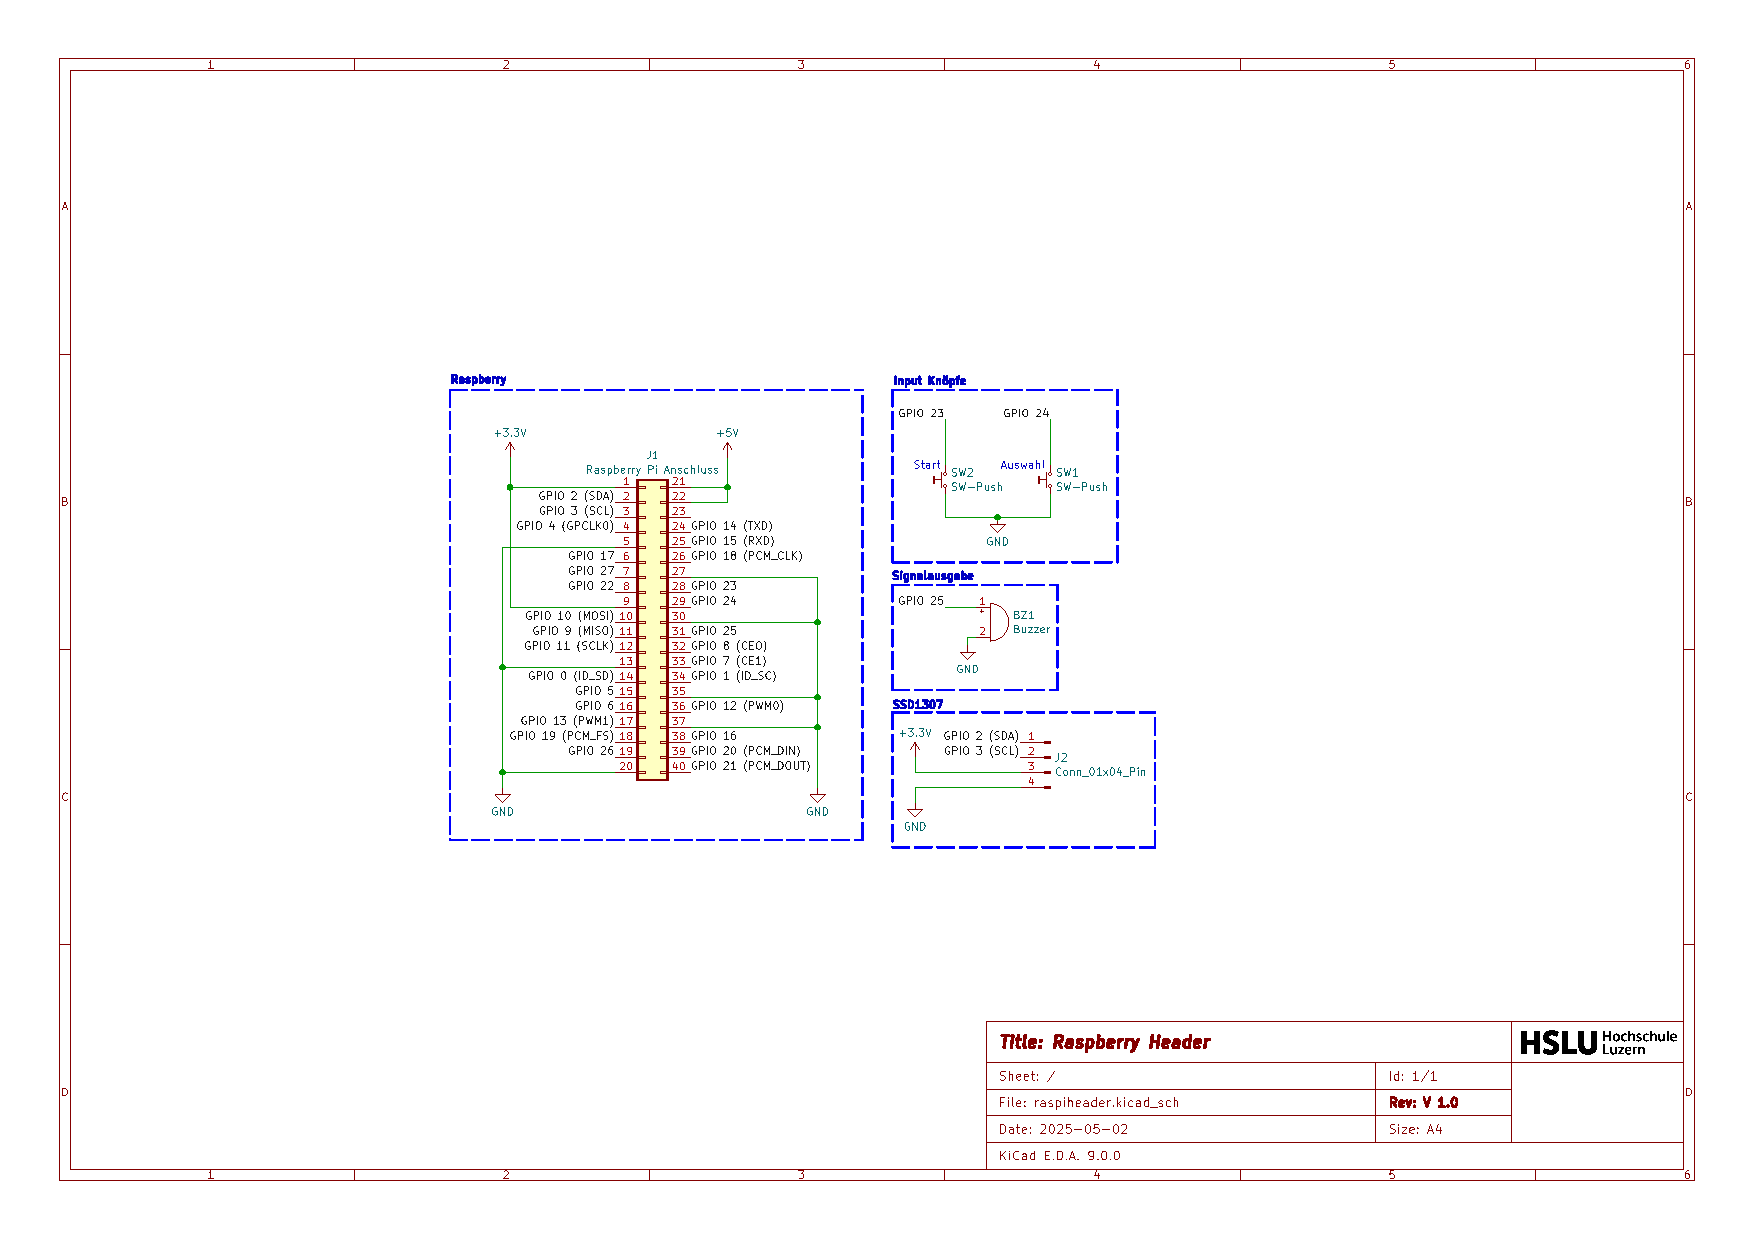
\includegraphics[width=\linewidth, trim=7.5cm 6cm 10cm 6cm, clip]{assets/ET/PCB/raspiheader.pdf}
    \caption{Raspberry Pi HAT Schema}
    \label{fig:raspiheader-schema}
\end{figure}

\begin{figure}[H]
    \centering
    \begin{subfigure}[t]{0.49\textwidth}
        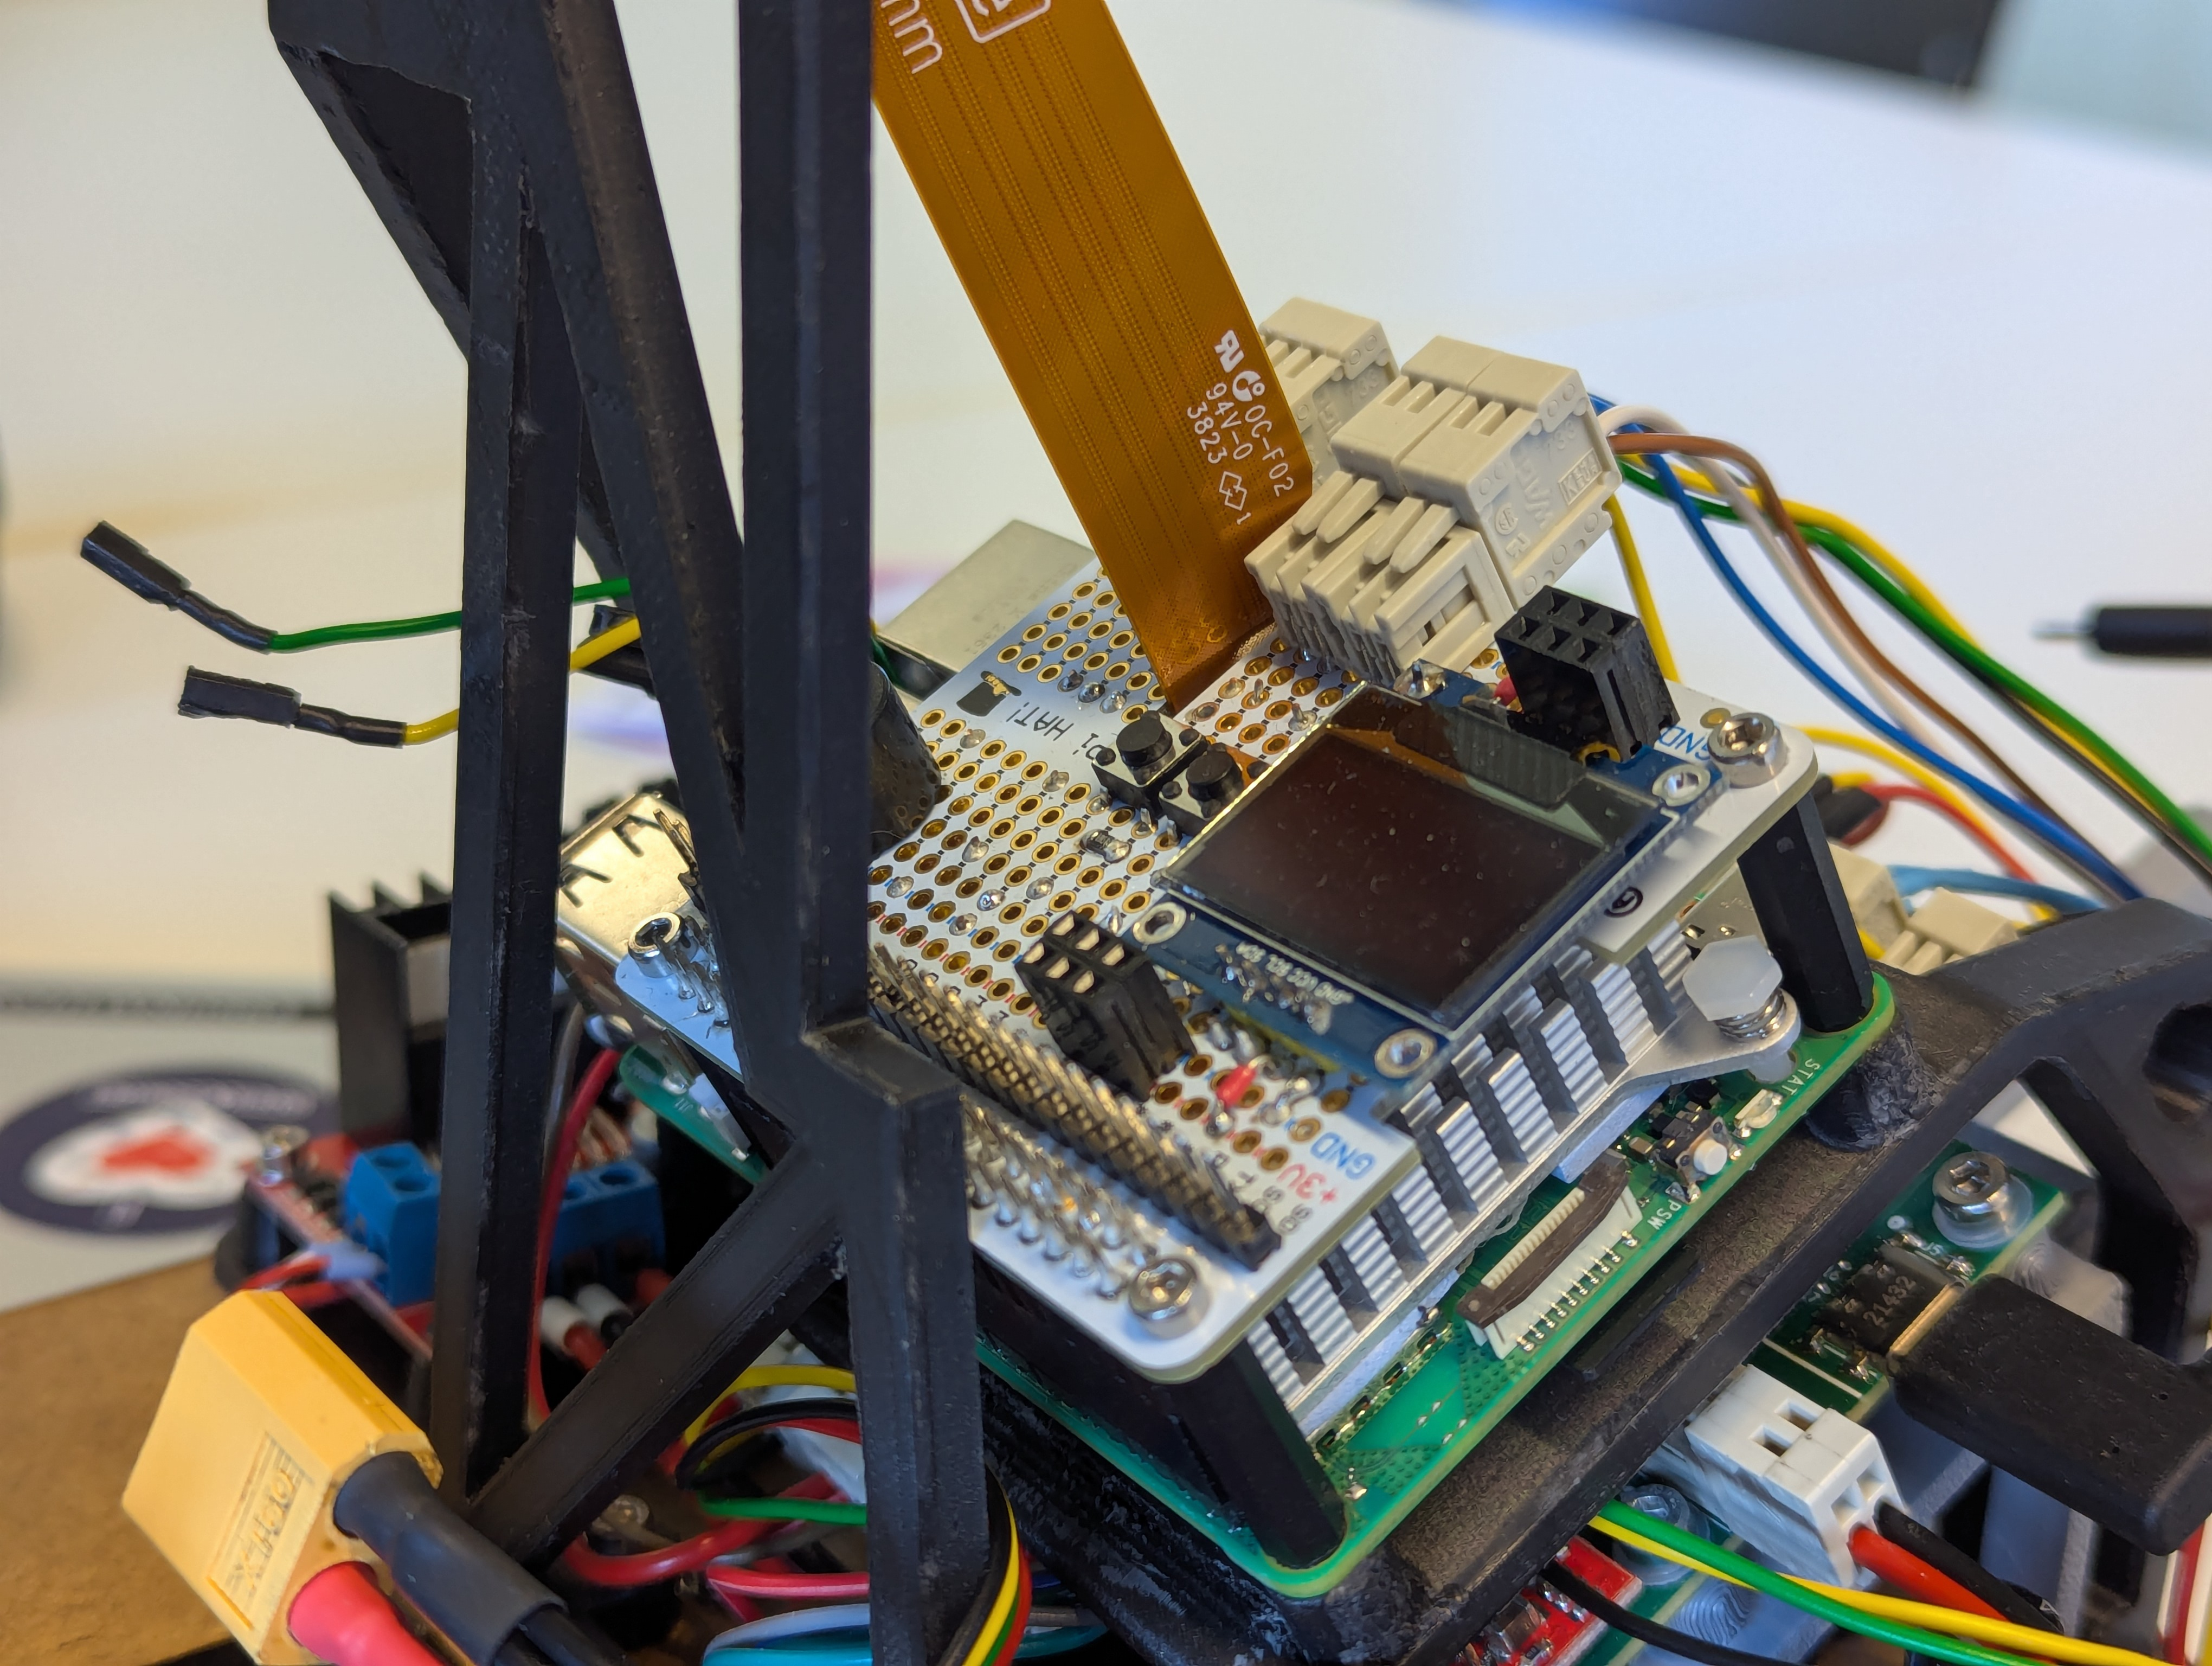
\includegraphics[width=\linewidth]{assets/IT/peripherie/raspi-hat_1.jpg}
    \end{subfigure}
    \hfill
    \begin{subfigure}[t]{0.49\textwidth}
        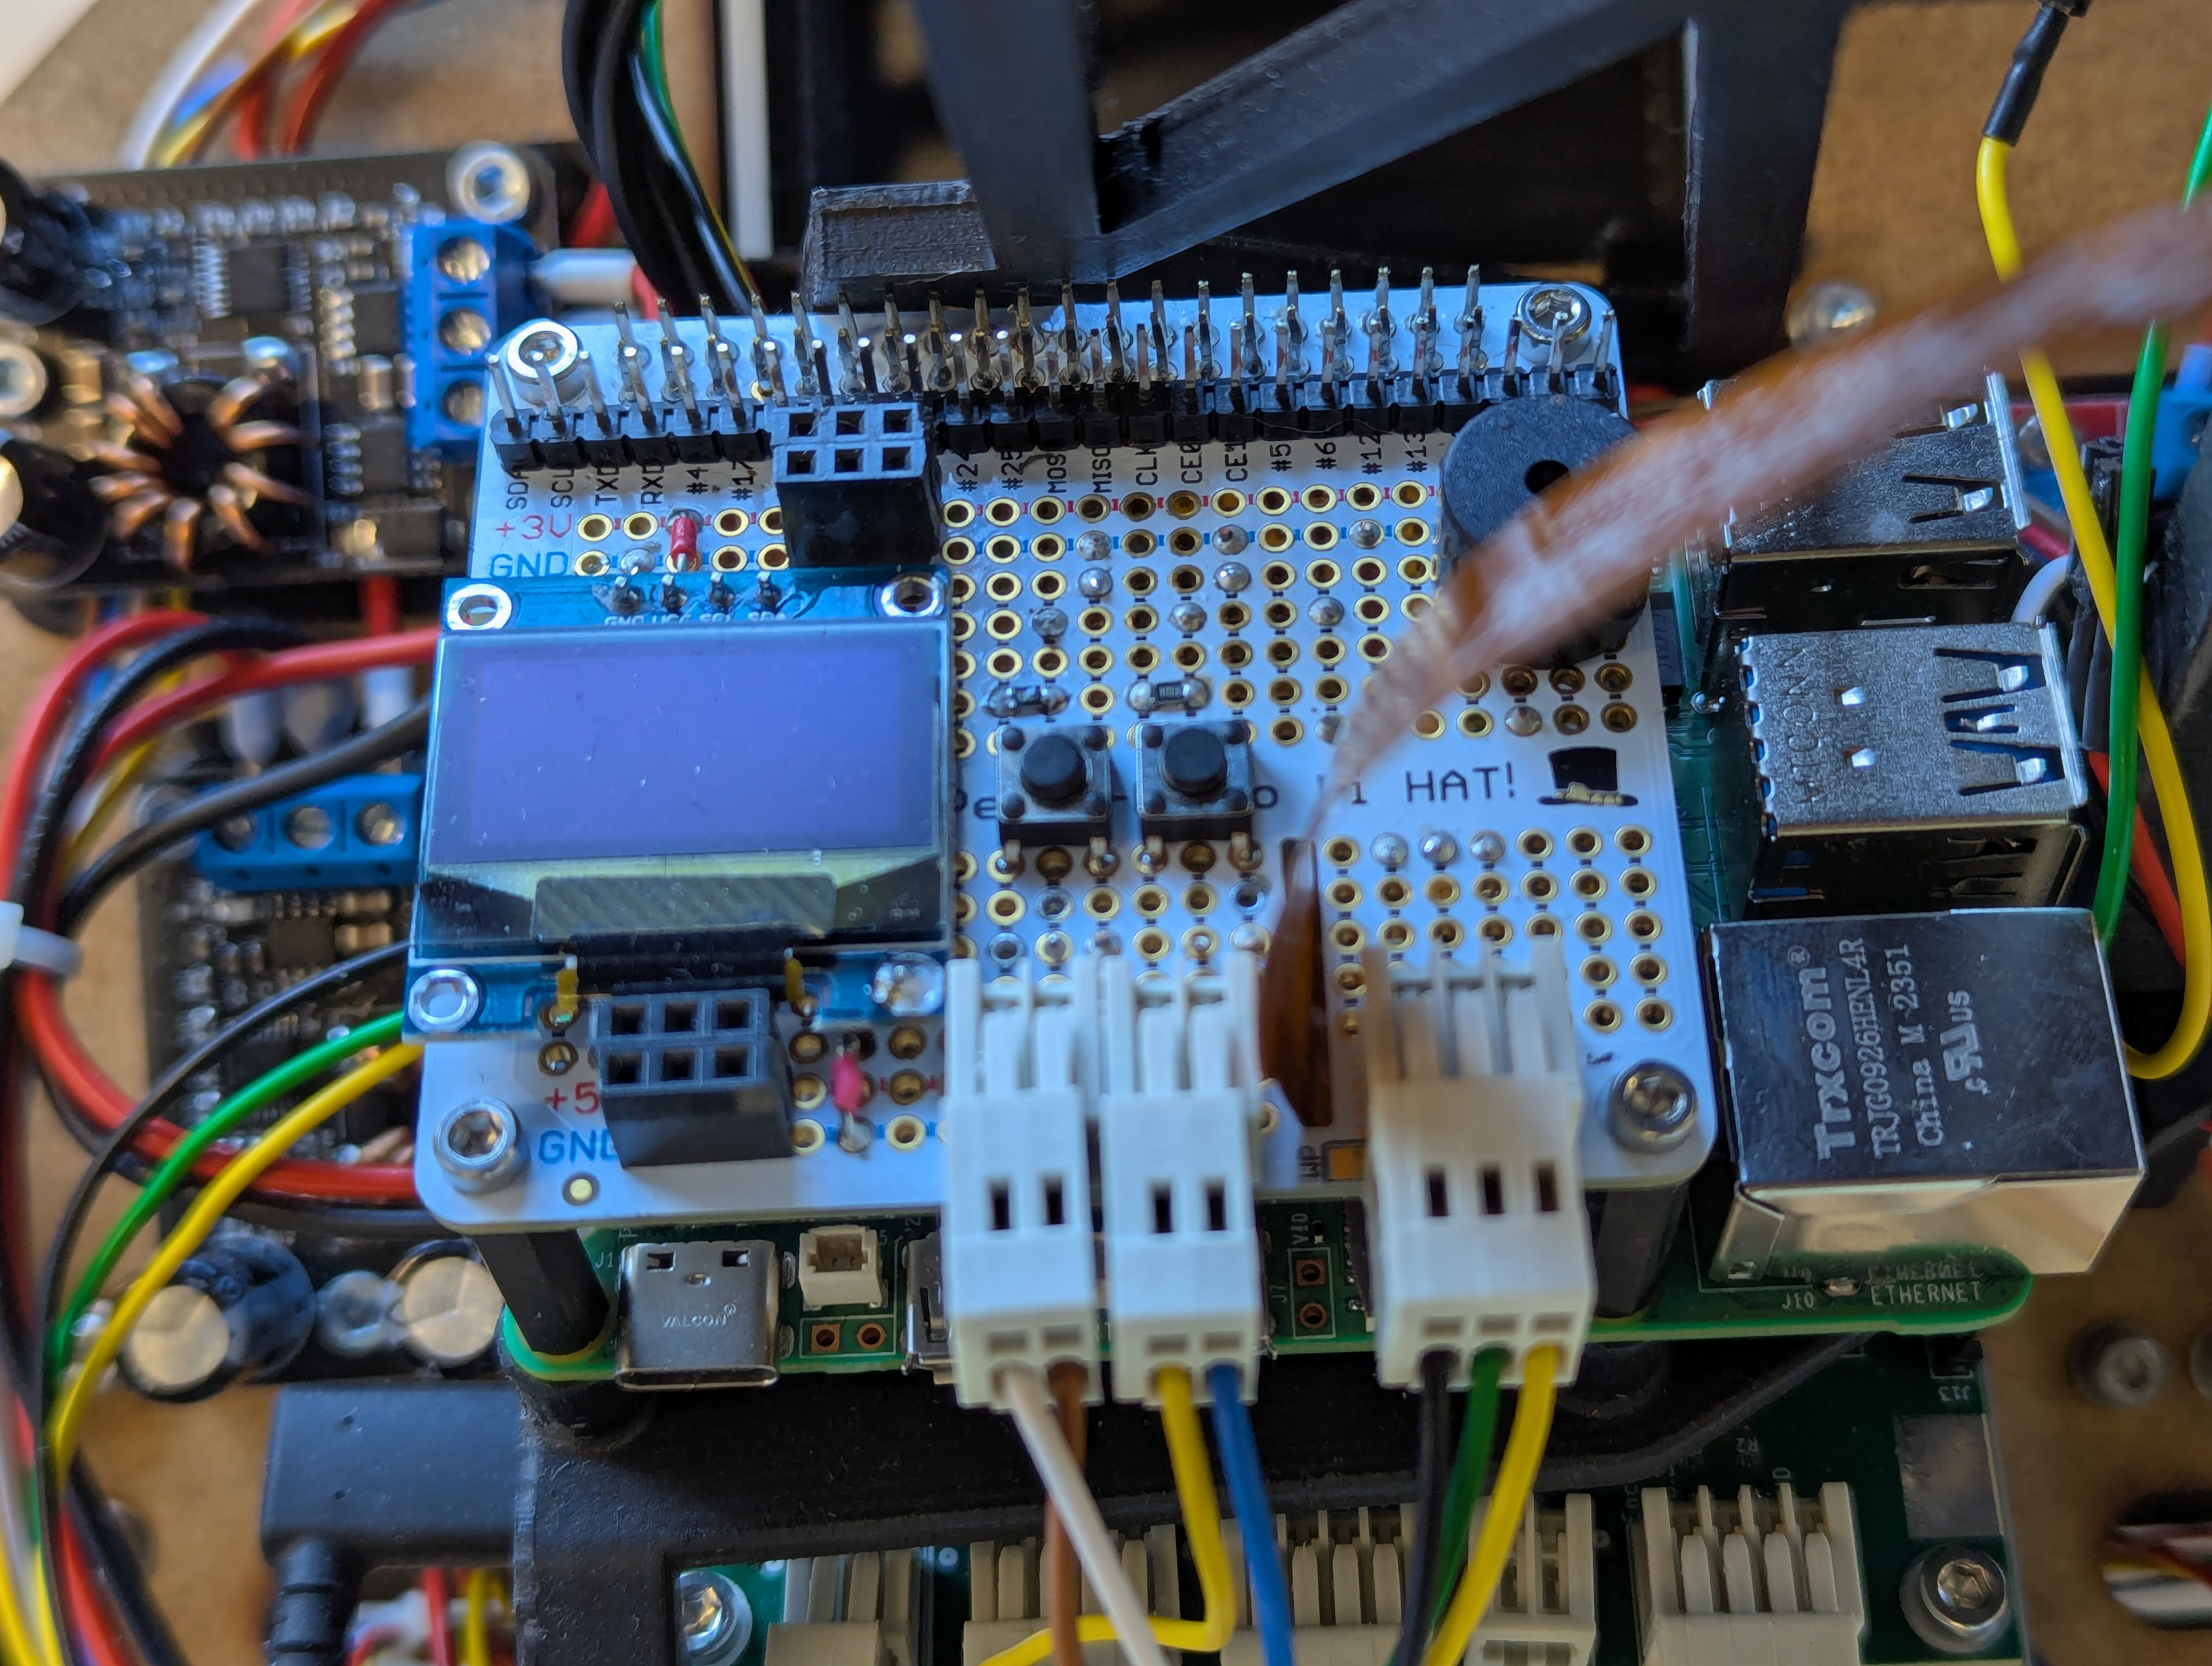
\includegraphics[width=\linewidth]{assets/IT/peripherie/raspi-hat_2.jpg}
    \end{subfigure}
    \caption{Raspberry Pi HAT zusammengebaut}
    \label{fig:raspiheader-assembly}
\end{figure}

Die Software dieser Komponenten wird direkt in Python auf dem Raspberry Pi umgesetzt. Nachfolgend in Abbildung \ref{fig:peripherie-classdiagramm} ist das Klassendiagramm ersichtlich. Es gibt einen RealPeripherieConnector, welcher von BaseConnector erbt, und die Hardwarefunktionen, wie Buttons und Buzzer, übernimmt. Zusätzlich gibt es einen MockPeripherieConnector, welcher zum Einsatz kommt, wenn kein GPIO zur Verfügung steht. Dieser simuliert die Ein- und Ausgabe auf dem Terminal. Somit kann stets der Programmcode auf dem PC ausgeführt werden, wo keine über GPIO verbundene Buttons und Buzzers verfügbar sind.

\begin{figure}[H]
    \centering
    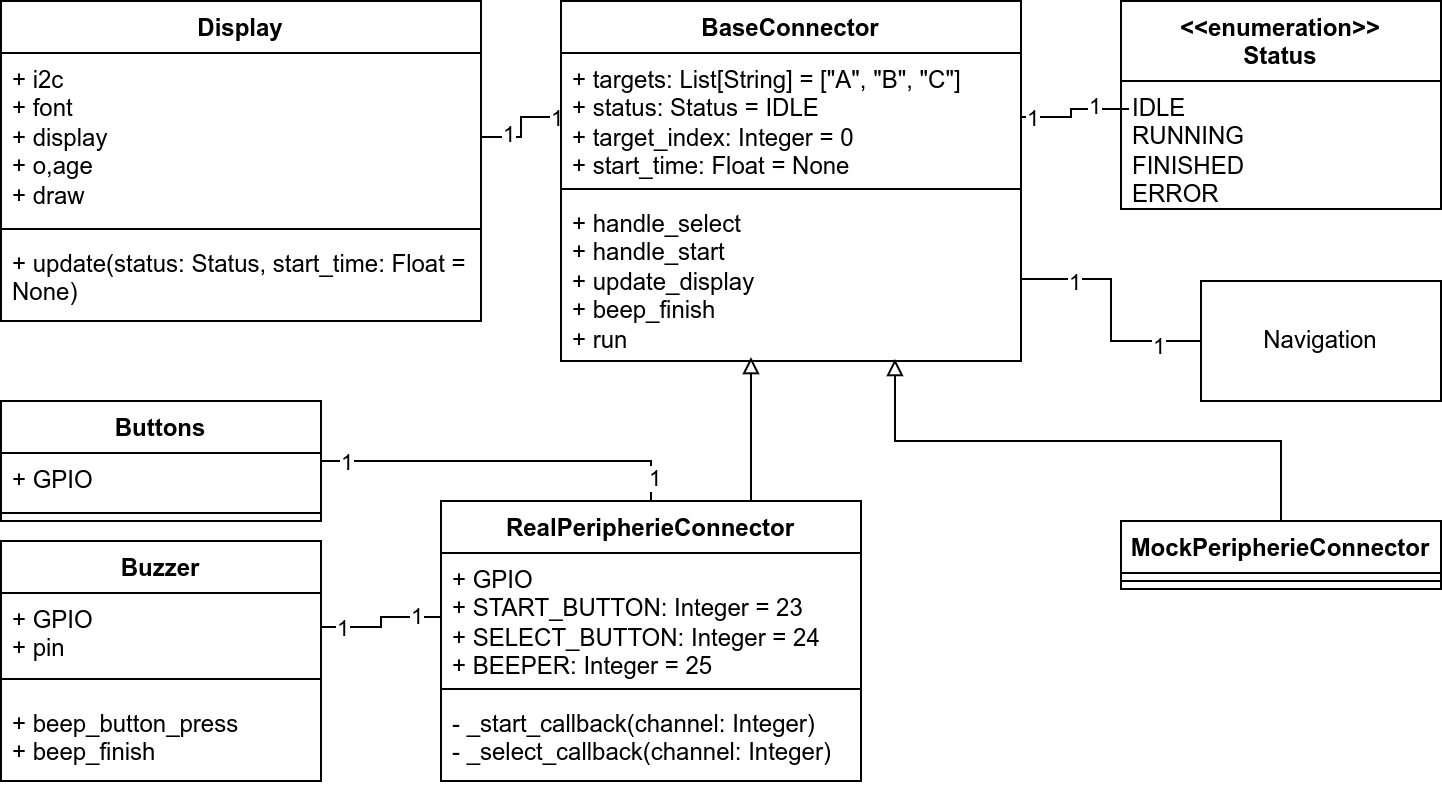
\includegraphics[width=\linewidth]{assets/IT/robot-sw-architecture-peripherie.png}
    \caption{Raspberry Pi HAT Klassendiagramm}
    \label{fig:peripherie-classdiagramm}
\end{figure}

\subsubsection{Peripherie Eingabe}
\label{zieleingabe}

\textbf{Zielknopf}

Die Zieleingabe wird verwendet, um vor dem Start den geforderten Zielknoten auszuwählen. Bei Knopfdruck werden die möglichen Zielknoten auf dem Display durchgeschaltet in der Reihenfolge A --> B --> C und dann wieder von vorne. So wird nur ein Taster benötigt, um zwischen den drei Zielen zu wechseln. Das Gewählte Ziel ist stets im Display (Kapitel \ref{peripherie-display}) ersichtlich.

\textbf{Startknopf}

Der zweite Taster ist der Startknopf. Dieser wird nach der Eingabe des Zielknoten gedrückt. Nach einer kurzen Wartezeit wird der Start initialisiert und der Roboter fängt an den Graphen in Richtung des Zielknotens zu traversieren.

Durch die einfache Zweitaster-Bedienung, und das ablesbare Display ist das Aufstellen sowie wählen des Zielknoten sehr gut unter 1 Minute möglich. Das Risiko 4 (1 Minute reicht nicht, siehe Tabelle \ref{table:risks}) kann somit vermindert werden.

\subsubsection{Peripherie Ausgabe}

\textbf{Display}\label{peripherie-display}

Das Display zeigt stets den aktuellen gewählten Zielknoten an, so kann einfach überprüft werden, welcher Zielknoten gewählt wird, bevor der Roboter gestartet wird. 
Zusätzlich wird der Status sowie die Laufzeit des Roboters dargestellt. Dadurch muss nicht separat eine Stoppuhr verwendet werden. Die Laufzeit wird automatisch beim Erreichen des Zielknotens gestoppt und bleibt ablesbar.

TODO LUKAS: insert image of Display\\
TODO ALINA: Take image of each state of the display (IDLE, RUNNING, FINISHED)

\begin{figure}[H]
    \centering
    \begin{subfigure}[t]{0.30\textwidth}
        
\includegraphics[width=\linewidth]{assets/placeholder.png}
    \caption*{Status: IDLE}
    \end{subfigure}
    \hfill
    \begin{subfigure}[t]{0.30\textwidth}
        
\includegraphics[width=\linewidth]{assets/placeholder.png}
    \caption*{Status: RUNNING}
    \end{subfigure}
    \hfill
    \begin{subfigure}[t]{0.30\textwidth}
        
\includegraphics[width=\linewidth]{assets/placeholder.png}
    \caption*{Status: FINISHED}
    \end{subfigure}
    \caption{Raspberry Pi Display}
    \label{fig:raspiheader-display}
\end{figure}


\textbf{Buzzer}\label{peripherie-buzzer}

Der Buzzer ertönt, sobald der Zielknoten erreicht wurde. Somit wird dem Bediener und Publikum vermittelt, dass der Roboter seine Traversierung beendet hat und sich am Zielknoten befindet.
